\documentclass[11pt]{article}
\usepackage{setspace}
\usepackage{graphicx}
\usepackage{amsmath}
\RequirePackage{hyperref}

\setstretch {1.25} 
\usepackage{geometry}
\geometry{papersize={21cm,29.7cm}}
\geometry{left=2.5cm,right=2.5cm,top=3cm,bottom=3cm}
\usepackage{fancyhdr}
\usepackage{listings}
\usepackage{color}
\usepackage{gensymb}
\usepackage{multicol}
%\usepackage{lastpage}
%\usepackage{showframe}

\usepackage[normalem]{ulem}
\definecolor{mygreen}{RGB}{28,172,0} % color values Red, Green, Blue
\definecolor{mylilas}{RGB}{170,55,241}
\definecolor{black}{rgb}{0,0,0}
\definecolor{olivegreen}{RGB}{112,161,71}
\definecolor{lakeblue}{RGB}{0,127,255}
\definecolor{orange}{RGB}{255,139,0}
\definecolor{purple}{RGB}{102,0,255}
\pagestyle{fancy}

\fancyhf{}
\lhead{\small Team \#41523}
\rhead{\small Page \thepage\ of \pageref{lastpage}}

%\lhead{\author}
%\chead{\date}
\lfoot{}
%\cfoot{\thepage}
\rfoot{}
\renewcommand{\headrulewidth}{0.4pt}
\renewcommand{\headwidth}{\textwidth}
\renewcommand{\footrulewidth}{0pt}
\newcommand{\alert}[1]{{ \color{purple} [{#1} ]}}

\newcommand{\vect}[1]{\mathbf{#1}}

\DeclareMathOperator*{\argmin}{arg\,min}
\DeclareMathOperator*{\argmax}{arg\,max}


\title{CasPPonNET: A predictive method to model the dynamics and control of Ebola }
\author{Team 41523}
\date{\today}
\begin{document}
	\maketitle
	\lstset{language=Matlab,%
	    %basicstyle=\color{red},
	    breaklines=true,%
	    morekeywords={matlab2tikz},
	    keywordstyle=\color{blue},%
	    morekeywords=[2]{1}, keywordstyle=[2]{\color{black}},
	    identifierstyle=\color{black},%
	    stringstyle=\color{mylilas},
	    commentstyle=\color{mygreen},%
	    showstringspaces=false,%without this there will be a symbol in the places where there is a space
	    numbers=left,%
	    numberstyle={\tiny \color{black}},% size of the numbers
	    numbersep=9pt, % this defines how far the numbers are from the text
	    emph=[1]{for,end,break},emphstyle=[1]\color{red}, %some words to emphasise
	    %emph=[2]{word1,word2}, emphstyle=[2]{style},    
	}
	
\section*{Abstract}
The world has been suffering from the Ebola virus disease (EVD) since March 2014. Recent days, a new round of outbreaks happened in West Africa. Imagine that we already have advanced medication for Ebola, but how can we develop a combination of optimal strategies to defeat Ebola in the most efficient and feasible ways?

We adopted a two-step framework to solve the problem. First, we built a predictive model to describe the spread of Ebola. Unlike traditional epidynamics model such as SIHR, we considered the effect of underlying network of the disease transmission based on geographical locations and population flow. We used a cascaded Poisson Process on the network, dubbed \emph{CasPPonNet} to model the disease diffusion and progress. Hyper parameters λ1 and λ2 are used to control the ratio of transmission from the same location and other locations, and are learned from data.

Not only the number of new cases can be predicted precisely, but also outbreaks in new areas can be predicted. Secondly, we used the precious information our model yield to design theoretical optimal drug and vaccine delivery strategies. 

Results from experiments on simulated data are proposed to demonstrate the performance of our model. Compared with baseline strategies, our strategy is better on both short term and long term goals. Based on our model and real-world data, we concluded Freetown(SL), Conakry(GN), Western rural(SL) and Port Loko(SL) are in urgent need of medicine and Dubreka(GN), Forecariah(GN) and Western rural(SL) are in need of vaccination now. We also determined the critical value for speed of manufacturing drug to bring the disease under control.



\section*{Keywords}
Cascaded Poisson Process, Epidemic diffusion network, Epidemic control


\newpage


\tableofcontents

\newpage





\section{Introduction}
\subsection{Background}




The Ebola virus causes an acute, serious illness which is often fatal if untreated. 

The current outbreak in west Africa, (first cases notified in March 2014\footnote{As the first case is observed in March 2014, we use the $\Delta t$ from a certain time to March 2014 to mark the progress of Ebola spread in the rest of the paper} ), is the largest and most complex Ebola outbreak since the Ebola virus was first discovered in 1976. There have been more cases and deaths in this outbreak than all others combined. 

The most severely affected countries, Guinea, Sierra Leone and Liberia have very weak health systems, lacking human and infrastructural resources, having only recently emerged from long periods of conflict and instability. On August 8, the WHO Director-General declared this outbreak a Public Health Emergency of International Concern.


\begin{figure}[hbtp]
\begin{center}
  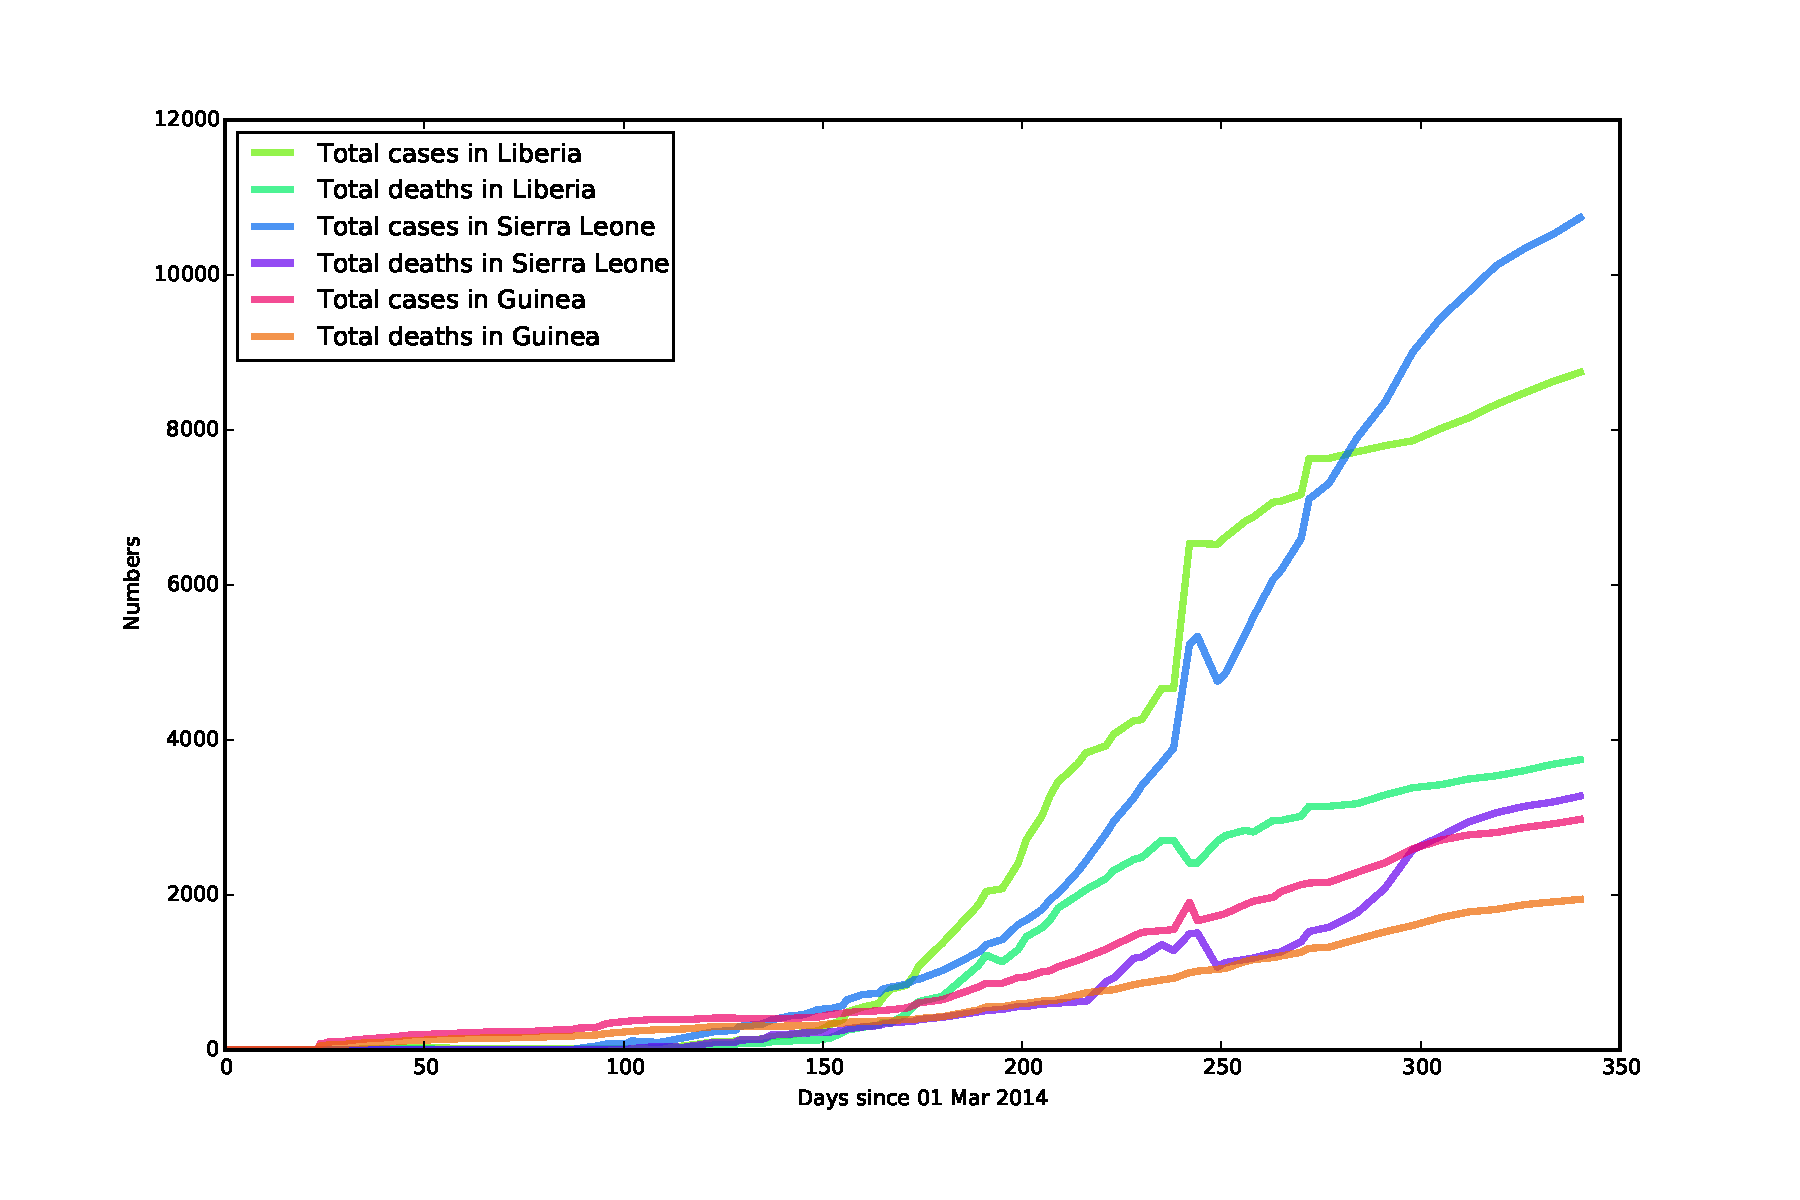
\includegraphics[width=4in]{graph/bstats.pdf}
  \caption{General statistics of Ebola outbreak in 2014}
  \label{stats}
\end{center}  
\end{figure}

Fig.~\ref{stats} shows the basic statistics of the Ebola outbreak in 2014. This is the cumulative cases and deaths in the three countries where the outbreak is the severe.\footnote{The hump of the curve origin from the inconsistency of the data source, it changed on Nov 12 2014.}



\subsection{Transmission}

It is thought that fruit bats of the Pteropodidae family are natural Ebola virus hosts. Ebola is introduced into the human population through close contact with the blood, secretions, organs or other bodily fluids of infected animals such as chimpanzees, gorillas, fruit bats, monkeys, forest antelope and porcupines found ill or dead or in the rainforest.


Ebola then spreads through human-to-human transmission via direct contact (through broken skin or mucous membranes) with the blood, secretions, organs or other bodily fluids of infected people, and with surfaces and materials (e.g. bedding, clothing) contaminated with these fluids.

It is reported that \cite{merler2015spatiotemporal}, 72\%  of infections occurred in households or in the general community , 17.5\% in hospitals, and 10.4\% at funerals. This observation is important for our modelling.

Human-to-human transmission gives rise to the wide spread such disease. It has spread between countries starting in Guinea then spreading across land borders to Sierra Leone and Liberia, by air (1 traveller only) to Nigeria, and by land (1 traveller) to Senegal.\cite{ebolanew}

Figure.~\ref{cities} shows the location of Ebola infected areas. We also got the geological location and other information such as population for the purpose of model calibration.

\begin{figure}[hbtp]
\begin{center}
  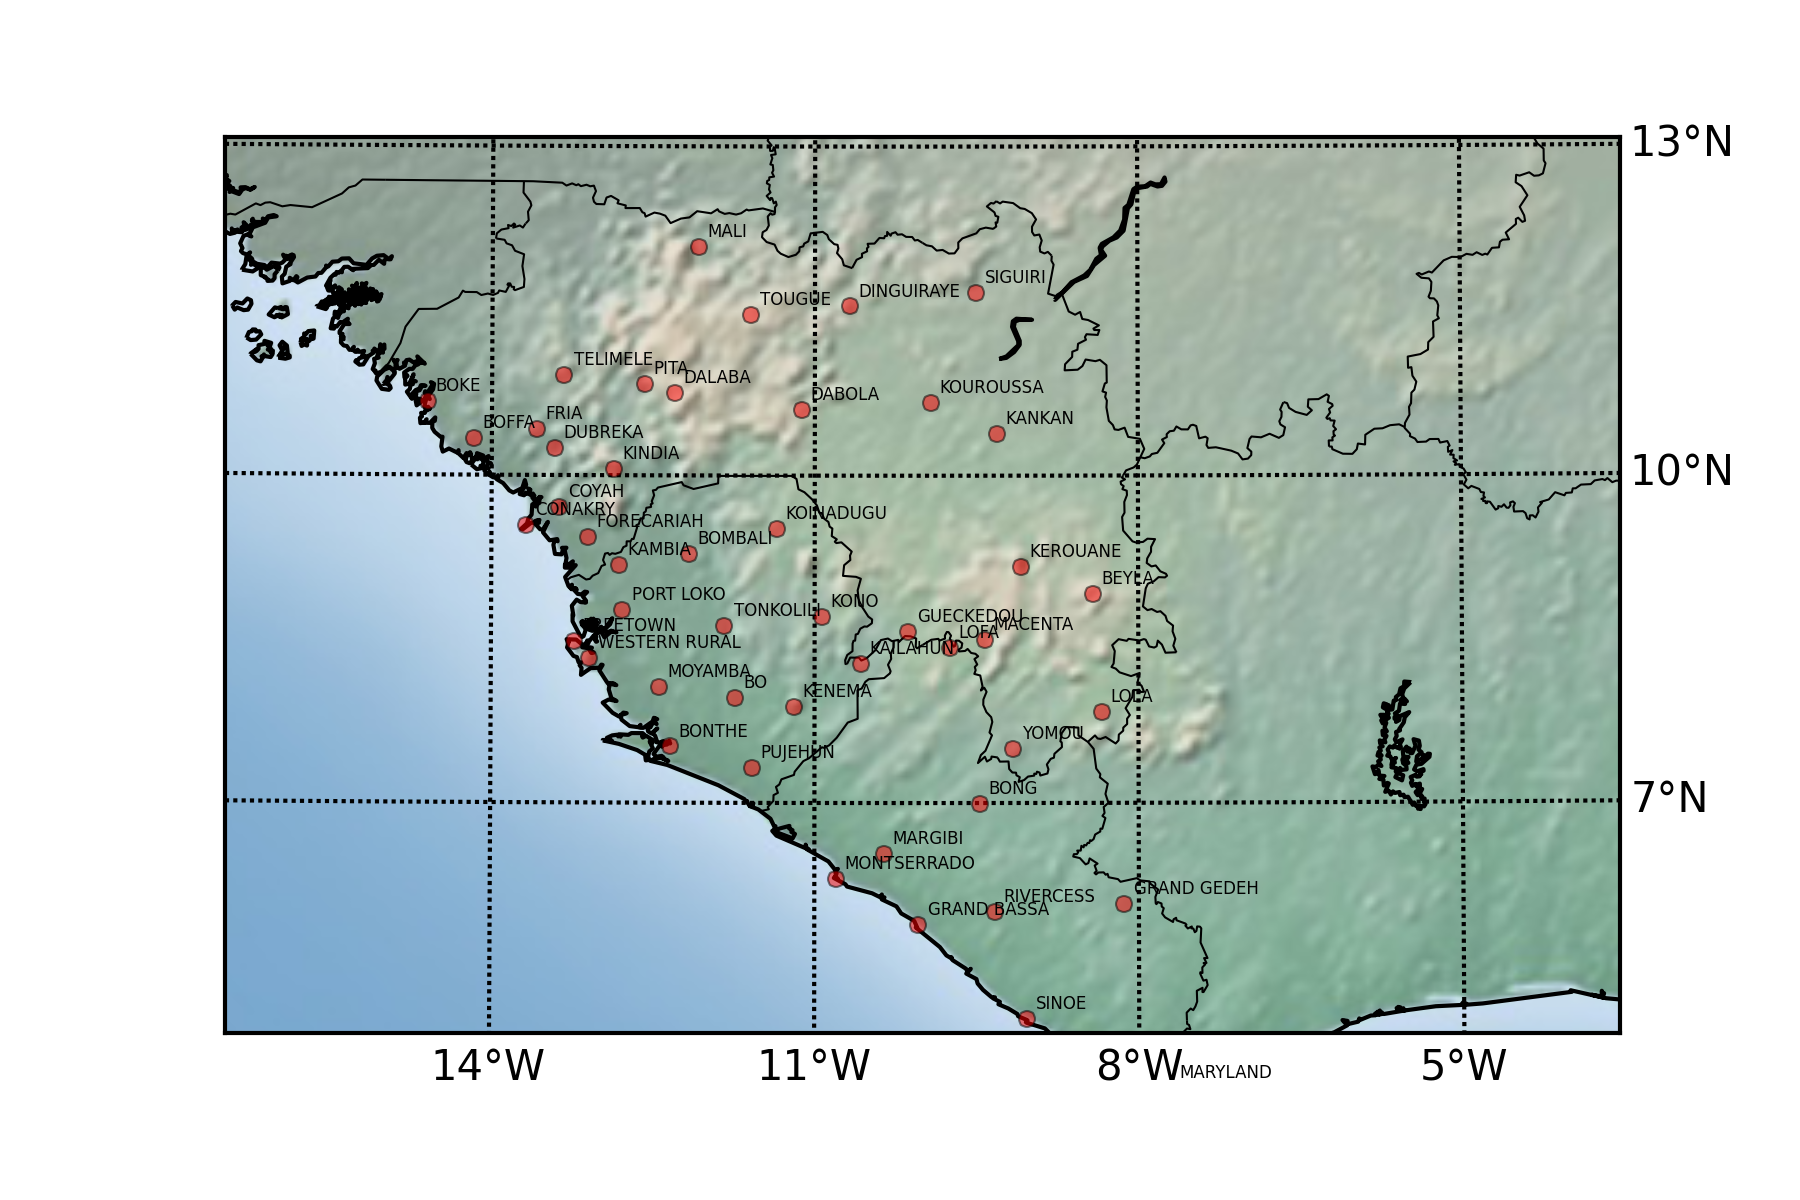
\includegraphics[width=4in]{graph/map3.png}
  \caption{Location of Ebola infected cities}
  \label{cities}
\end{center}  
\end{figure}

According to the observation of the outbreak data in Fig.~\ref{spread} in the Appendix , we found there exists a strong correlation  between infected areas in time. This observation validated that Ebola spread between countries on the land.



\subsection{Medication}

Supportive care-rehydration with oral or intravenous fluids and treatment of specific symptoms, improves survival. There is as yet no proven treatment available for EVD. However, a range of potential treatments including blood products, immune therapies and drug therapies are currently being evaluated. No licensed vaccines are available yet, but 2 potential vaccines are undergoing human safety testing.

However, in the modelling, we assume medicine and vaccines are found for treating Ebola. The mechanism of these two different types of medication methods plays different roles in controlling Ebola.


\section{Problem Formulation}



\subsection{Problem Restatement}

The world medical association has announced that their new medication could stop Ebola and cure patients whose disease is not advanced. 

The goal is to bring Ebola under control and ultimately, eliminate this disease. To achieve this goal, a sensible model has to be built, taking not only the spread of the disease, the quantity of the medicine needed, possible feasible delivery systems, locations of delivery, speed of manufacturing of the vaccine or drug into consideration. Then use this model to optimize the eradication of Ebola.

It is natural to break this problem into two parts:
\begin{itemize}
\item
 The first part focuses on the Ebola itself. For this part, we need to build a model to describe how Ebola spreads and progresses. 
\item
The second part is to build an optimization model to optimize the eradication of Ebola based on the intrinsic properties of Ebola. 

\end{itemize}

\subsection{Challenges}

Previous research focuses on the statistical level of disease modelling\cite{anderson1992infectious}\cite{lekone2006statistical}\cite{ivorra2014codis}\cite{team2014ebola}\cite{chowell2014transmission}   , thus detailed plan is not easily made from that. So it is challenging to build a fine grind model to assist detailed region-level healthcare plan-making.

The second challenge lies in the spread of disease. Many a time only one traveller from one area to another will cause infection and disease spread in that new area. Traditional statistical models views the population in as a whole, thus they are not able to track such phenomenon. The challenge is to view different areas as a network and consider the effect of population migration\cite{basharpredicting} .


\section{Disease Modelling}
\label{dmodel}
\subsection{Assumptions}

For the transmission of the disease, we made several assumptions:

\begin{itemize}

\item The transmission of Ebola has a certain mechanism. We mainly consider the man-to-man transmission and ignore the transmission from the environment.

\item The flow of population is the mechanism of geographical spread of Ebola.

\item The transmission of Ebola will not happen beyond the nodes we consider and no new node will join our network in the time we concern.

\end{itemize}

For the controlling of the disease, we assume:

\begin{itemize}

\item There exists medicine that could cure patients whose disease is not advanced. 

\item Those people who got vaccinated are immune to the disease in the future.

\item Once cured, the patient has no chance to be infected again.

\end{itemize}

\subsection{Notations}


\begin{table}[hbtp]
\begin{center}
\begin{tabular}{|c|p{9cm} |}
\hline

Notations & Descriptions \\
\hline

$G$ & The network on which Ebola diffuses\\
\hline
$N_i$ & The nodes on the network, i.e regions on the land\\
\hline
$\sigma_{i,j}$ & The weights of edges on the network \\
\hline
$Po_{i}$ & Population of node(region) $i$ \\
\hline
  \multicolumn{2}{|c|}{Variables for SIHRonNET model} \\
\hline
$S_{i}$ & number of people in state S(suspected) on node $i$ \\

\hline
$I_{i}$ & number of people in state I(infected) on node $i$ \\
\hline

\hline
$H_{i}$ & number of people in state H(in hospital) on node $i$ \\

\hline
$\eta$ &  death rate of Ebola \\


\hline
$R_{i}$ & number of people in state R(removed) on node $i$ \\


\hline
  \multicolumn{2}{|c|}{Variables for CasPPonNET model} \\
\hline
$\mu_{i,t_k}$ & the intensity of Poisson Process on node $i$ in time window $t_k$ \\

\hline
$P_{i,t_k}$ & the number of new cases on node $i$ in time window $t_k$ \\


\hline
  \multicolumn{2}{|c|}{Variables for disease controlling} \\
\hline


$C_{i,t_k}$ & the number of people cured on node $i$ in time window $t_k$ \\

\hline
$V_{i,t_k}$ & the number of people vaccinated on node $i$ in time window $t_k$ \\

\hline
$\mu'_{i,t_k}$ & the intensity of Poisson Process after disease controlling on node $i$ in time window $t_k$ \\

\hline
$w_{c,i}$ & the weight of medicine on node $i$  \\

\hline
$w_{v,i,k}$ & the weight of vaccine on node $i$ in time window $t_k$ \\


\hline
\end{tabular}
\end{center}
\caption{Notations}
\label{testtable}
\end{table}


\subsection{Network Building}


When we consider the established models , we can see that some of them are based on statistics of either the total population\cite{althaus2014estimating} , which cannot describe the beginning of spatial spread perfectly. 

Other researches\cite{lewnard2014dynamics}, however, based their models on individual person. These models can work sometimes but cost a lot of time to simulate. These methods also leave a lot of parameters to calibrate. 

So we came up with our model of the network.

The Ebola infected countries are divided into areas based on its political divisions. We denote the areas as nodes, $N_i$. And there exist links between every two nodes. We assign a weight $\sigma_{i,j}$ on each edge to describe the `proximity' of two areas. 
 
Because we mainly consider the population flow, so we adopted the gravity model\cite{anderson2010gravity}\cite{karemera2000gravity} in economics to estimate the population flow between to areas.

$$\sigma_{i,j} = \frac{Po_i^{\beta_1}Po_j^{\beta_2}}{d_{i,j}^{\beta_3}}, i \neq j$$

We denote the population of node $i$ as $Po_i$ and the geological distance between node $i$ and node $j$. For simplification, we set:

$$\beta_1 = 1, \beta_2 = 1, \beta_3 = 2$$

This is commonly used in modelling population migration.

In order to calculate the distance between two nodes, we simply used the euclidean distance between two nodes.

We fetched the data of 55 infected areas. The link and the strength of links is visualized in Fig.~\ref{network}, and the area of circles stands for the population.

\begin{figure}[hbtp]
\begin{center}
  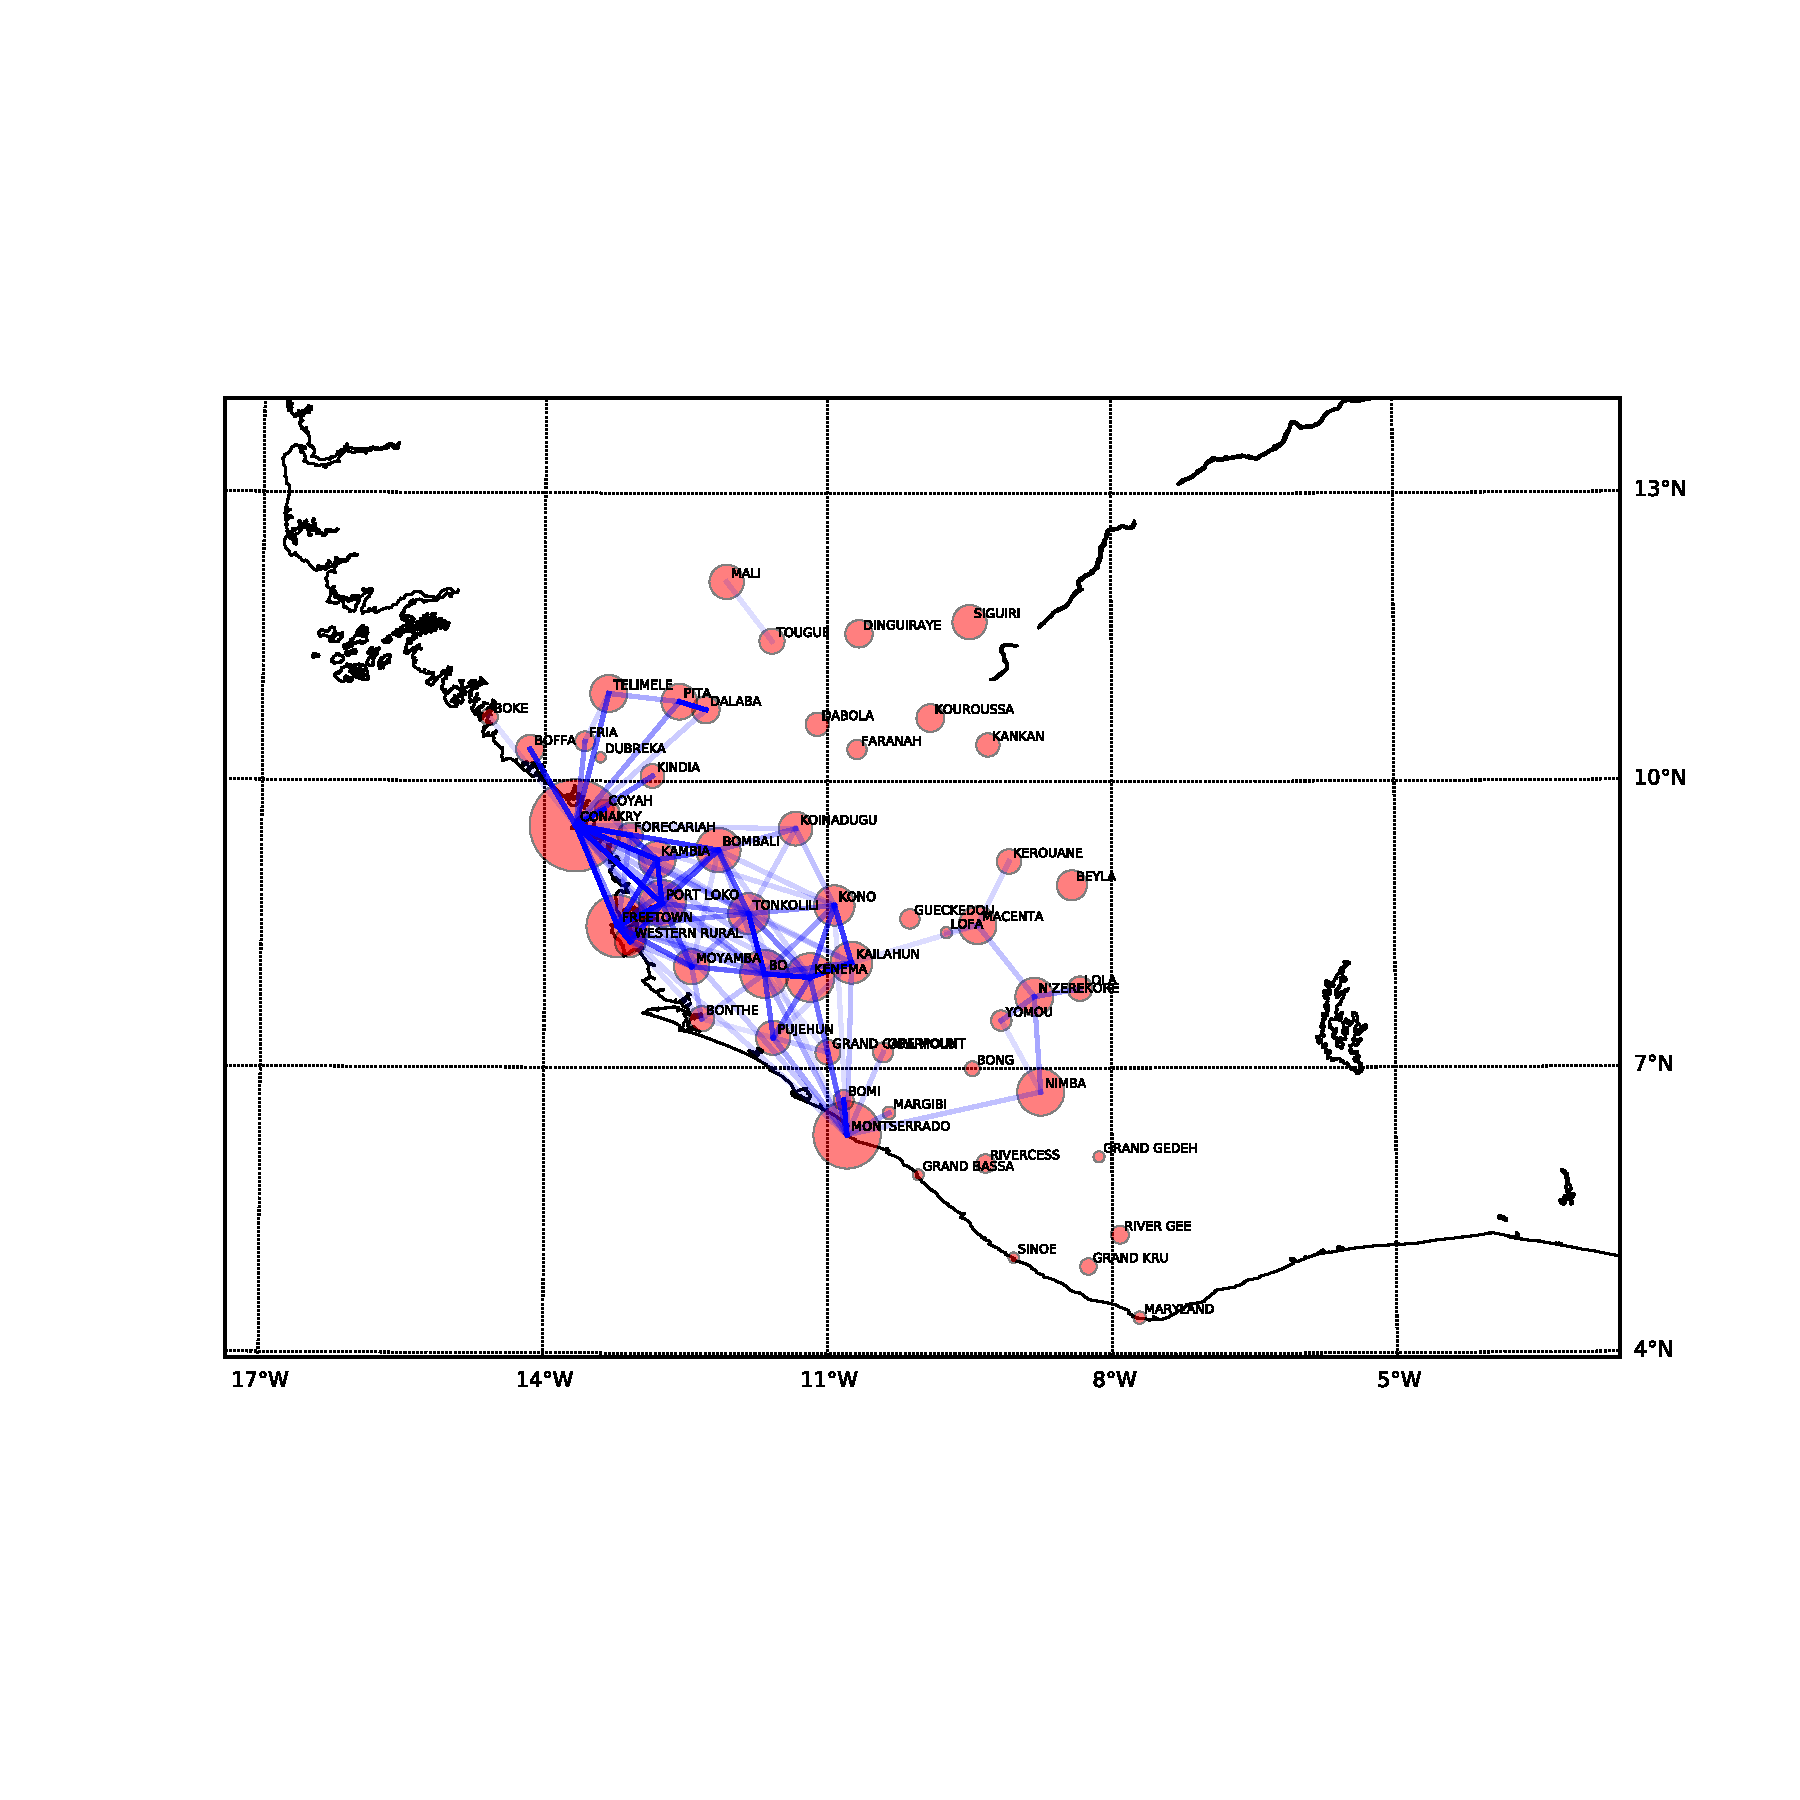
\includegraphics[width=4.5in]{graph/network2.pdf}
  \caption{Underlying network of population flow}
  \label{network}
\end{center}  
\end{figure}

\subsection{Differential equation model on the network :  SIHRonNET}

We proposed an assisted model based on the network structure and an assisted traditional SIR model.

Other assumptions have to be made. We classify the people into one of the following states:

\begin{itemize}
    \item S: Suspected, not infected but possible for infections
    \item I: Infected, but not go to hospital
    \item H: Infected, and in hospital
    \item R: Removed, recovered or passed away
\end{itemize}

For simplification, we assume the ratio of death or recover is constant and can be observed from statistical data.

\subsubsection{Differential Equation model without considering population flow}

$N$ denotes for the whole population. Because there are three main causes of infection, \emph{household transmission, clinical transmission, and funeral transmission}.

So the rate is proportional to three terms, corresponding to the three causes.

$$\frac{\mathrm{d}S}{\mathrm{d}t} = -\frac{\beta_1 S I}{N}-\frac{\beta_3 S H}{N}  - \frac{\beta_2 S }{N} \frac{\mathrm{d}D}{\mathrm{d}t} $$ 


$$\frac{\mathrm{d}I}{\mathrm{d}t} = \frac{\beta_1 S I}{N} +\frac{\beta_3 S H}{N}  + \frac{\beta_2 S }{N} \frac{\mathrm{d}D}{\mathrm{d}t} - kI$$ 

$$\frac{\mathrm{d}H}{\mathrm{d}t} = kI - \gamma H$$

$$\frac{\mathrm{d}R}{\mathrm{d}t} = \gamma H$$
Because the ratio of death or recover is constant and can be observed from statistical data,so 
$$D =\eta R. $$

\subsubsection{Differential Equation model with considering population flow}

The underlying network is the main dynamic of disease sprawling. 

For every node $V_i \in V$

$$\frac{\mathrm{d}S_i}{\mathrm{d}t} = -\frac{\beta_1 S_i I_i}{N_i}-\frac{\beta_3 S_i H_i}{N_i}  - \frac{\beta_2 S_i }{N_i} \frac{\mathrm{d}D_i}{\mathrm{d}t} + \sum_{j\in V,j\neq i} \theta(\sigma_{i,j} S_j - \sigma_{j,i} S_i) $$ 


$$\frac{\mathrm{d}I_i}{\mathrm{d}t} = \frac{\beta_1 S_i I_i}{N_i} +\frac{\beta_3 S_i H_i}{N_i}  + \frac{\beta_2 S_i }{N_i} \frac{\mathrm{d}D_i}{\mathrm{d}t} - kI_i + \sum_{j\in V,j\neq i} \theta(\sigma_{i,j} I_j - \sigma_{j,i} I_i)$$ 

$$\frac{\mathrm{d}H_i}{\mathrm{d}t} = kI_i - \gamma H_i$$

$$\frac{\mathrm{d}R_i}{\mathrm{d}t} = \gamma H_i$$
Because the ratio of death or recover is constant and can be observed from statistical data,so 
$$D_i =\eta R_i. $$




\subsubsection{Two step model calibration}
The first step of calibration is to determine the parameters for the overall data.

The parameters are $\beta_1,\beta_2,\beta_3, k,\gamma$.

Write the equations in matrix form.
$$\vec{x} =  \begin{pmatrix}
S\\I\\H
 \end{pmatrix}$$ 
 
 $$
 A =  \begin{pmatrix}
0 &-\beta_1 & -\beta_3-\beta_2\eta\gamma \\
0 &\beta_1 -k & \beta_3 + \beta_2 \eta\gamma \\
0 & k & -\gamma 
 \end{pmatrix}
 $$
 
 Considering the number infected is small comparing to the population. So $$S_i \approx N_i, $$
 
 $$\dot{\vec{x}} =  A  \vec{x}$$
 
 The roots of equation $|pI-A| = 0$ are:
 
 $$
 p_1 = 0
 $$
 
 $$
 p_{2,3} = \frac{-k+\beta_1 - \gamma \pm \sqrt{  (\beta_1 - \gamma - k)^2  - 4(\beta_1 - \gamma - mk + k\gamma) } }{2}
 $$
 
 
 The general solution is 
$$\psi = A\begin{pmatrix}
1\\0\\0
 \end{pmatrix}
 +B\begin{pmatrix}
-m\frac{p_2 + k}{p_2}\\ m \\ p_2 - \beta_1 + k
 \end{pmatrix}
 +C\begin{pmatrix}
-m\frac{p_3 + k}{p_3}\\ m \\ p_3- \beta_1 + k
 \end{pmatrix}
$$


From statistical data we set $\beta_1:\beta_2:\beta_3 = 2:2:1$

$$\beta_1 = 2\beta, \beta_2 = 2\beta,\beta_3 = \beta$$
 
 
 
We fit the data to the first $2/3$ data and get $$\beta = 0.0612$$ in Fig.~\ref{cfit}.

\begin{figure}[hbtp]
\begin{center}
  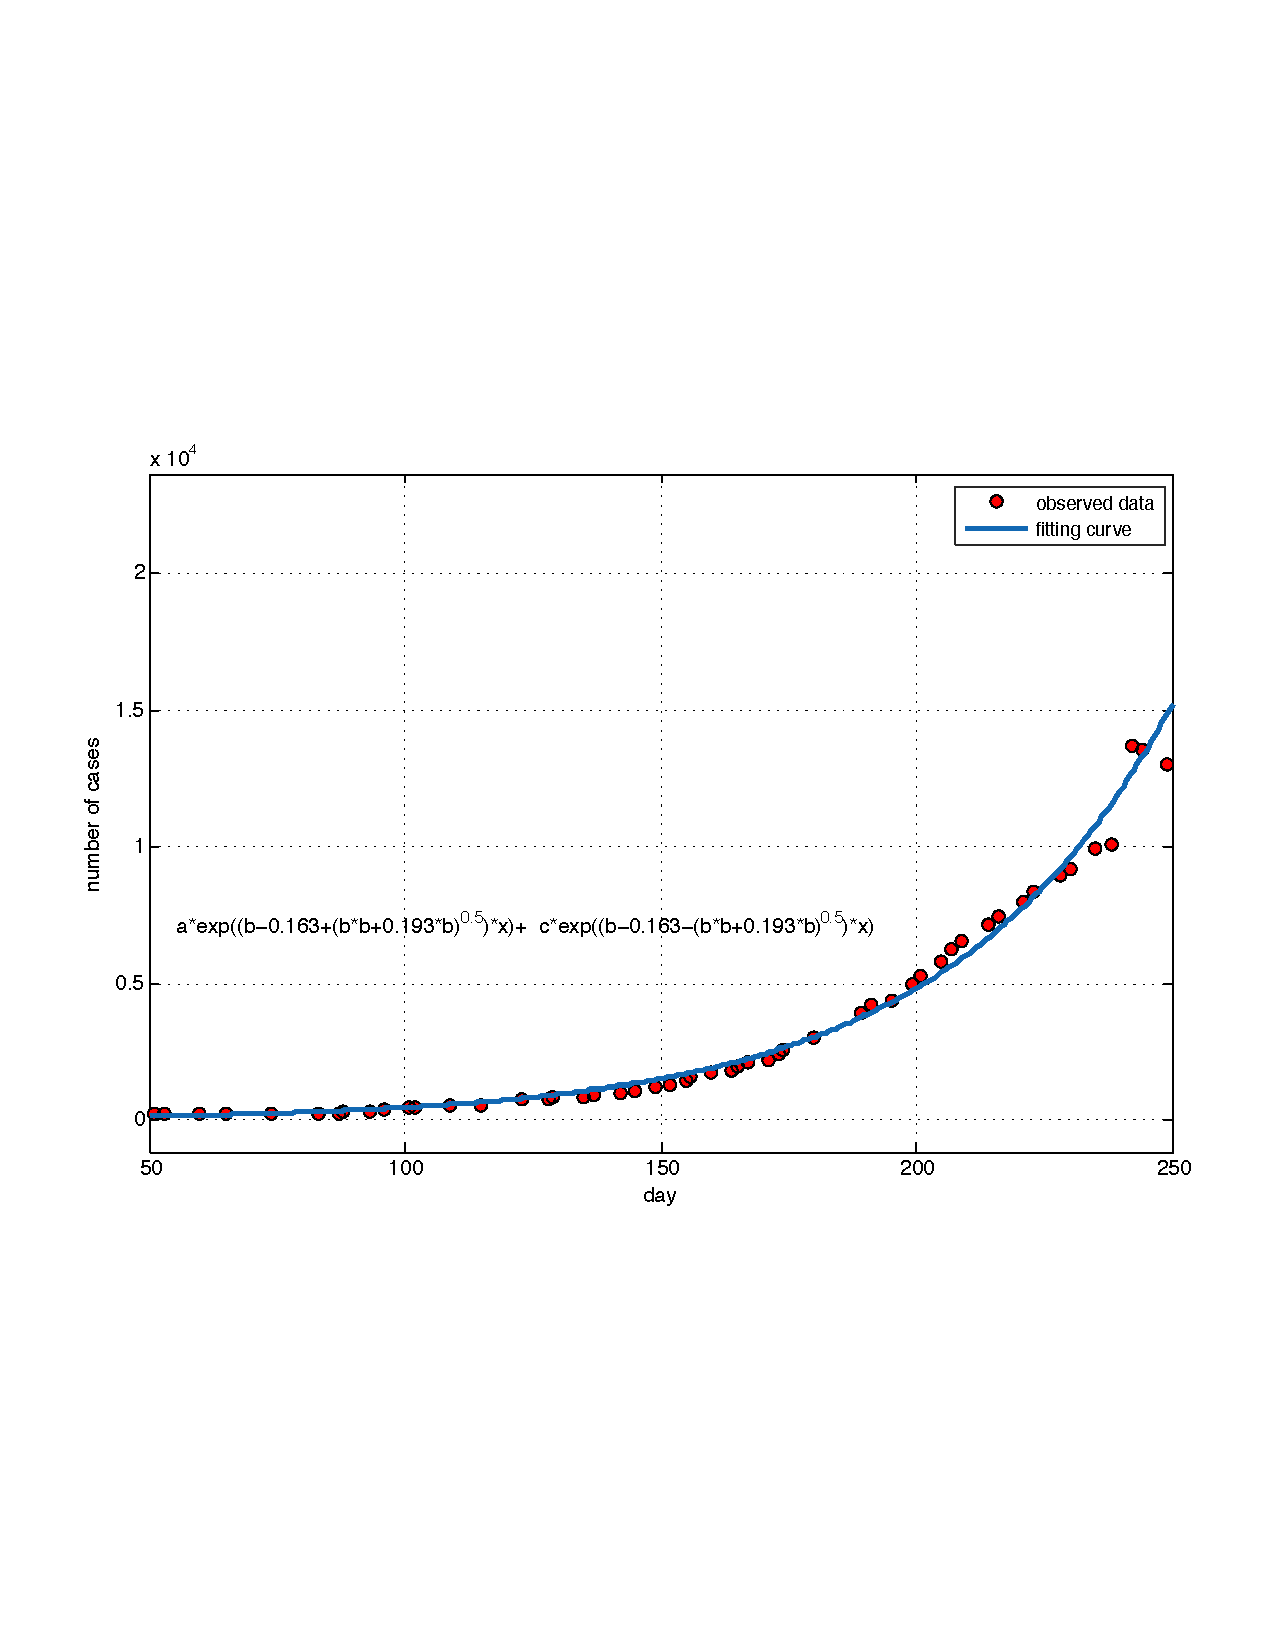
\includegraphics[width=4in]{graph/cfit.pdf}
  \caption{Estimate parameter $\beta$ }
  \label{cfit}
\end{center}  
\end{figure}




The second step of calibration considered the population flow. During the calibration, data of different times at different nodes is used as our initial conditions and after our simulation, we can obtain the prediction for new cases after a fixed time period. And the norm of prediction error can thus be gotten. Thus the best fitted theta can be considered as the one that make the prediction error smallest. The relationship between error and theta can be show as:

We can see that the best theta is about $$\theta = 0.3 \times 10^{-3}$$

Since $\theta$ is such a key parameter which we can conduct the influence ratio between node itself and its neighbourhood, we now give a short discussion. From the right side of second differential equation, we express the influence ratio as

$$
\frac{\sigma_{i,j} I_i}{\beta_1 \frac{S_i I_i}{N_i} } = =  \frac{\theta \sigma_{i,j} N_i}{\beta_1 S_i}
$$

We can estimate the ratio because we konw:

$$
\sigma_{i,j} \sim 10^0, N_i \sim S_i, \beta \sim 10^{-2}, \theta \sim 10^{-3}
$$

Thus the ratio is about $10^{-1}$, meaning that the influence given by a node itself is about $10^1$ times stronger than that obtained from its neighbours.

This ratio is critical to us since it models the geological spread of Ebola. 

\begin{figure}[hbtp]
\begin{center}
  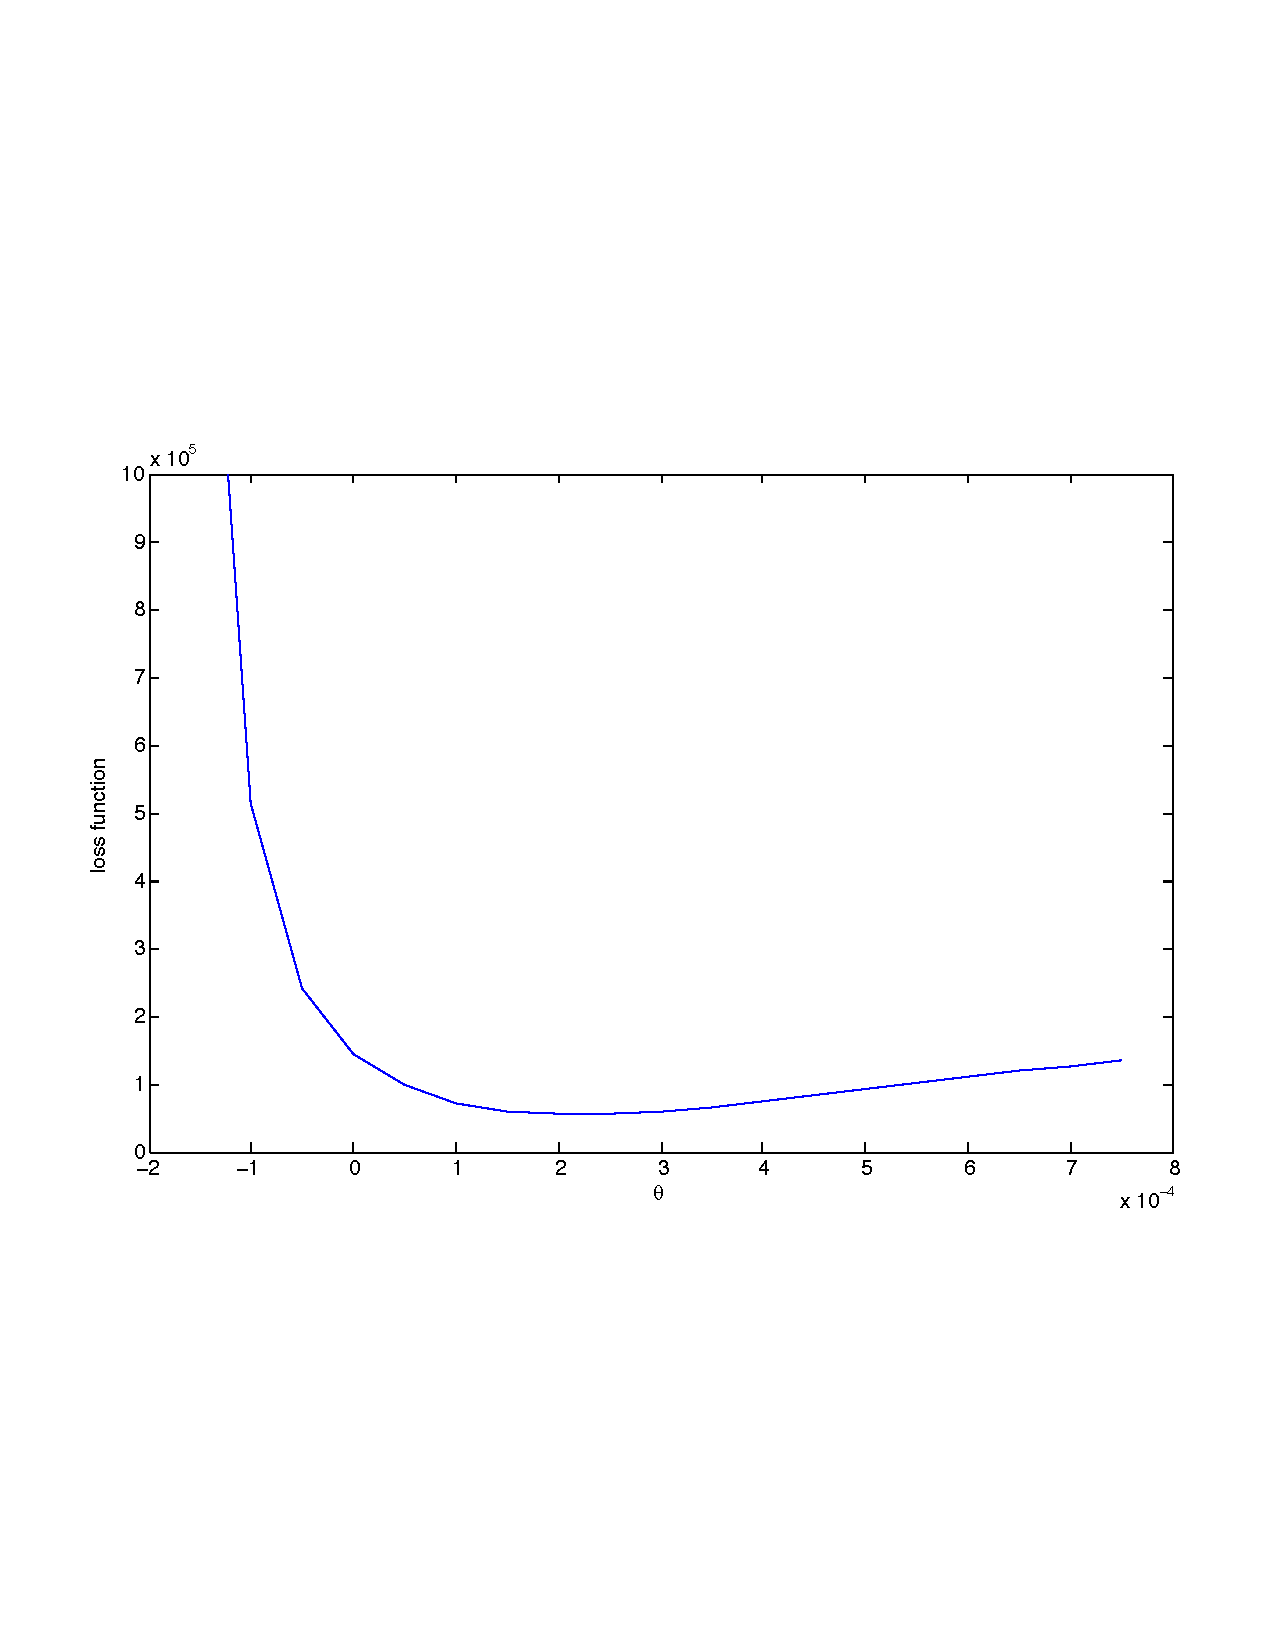
\includegraphics[width=4in]{graph/est3.pdf}
  \caption{Estimated $\theta$}
  \label{est}
\end{center}  
\end{figure}

\label{eth}

\subsubsection{Model Analysis}

During our modeling process using SIHRonNet model, some weakness of these differential model has been exposed clearly, which can be summarized in three aspects:
\begin{itemize}

\item Bad Timescale: SIHR model does make sense to describe the entire process of a disease outbreak, but its description to the beginning of an outbreak is trivial an exponential-like increase can't give us the detailed information we want.  
\item No Randomness:In theses models, all the interactions between different states of people is modelled using a proportional relationship, meaning that the model is based on statics. This erases the randomness, which is an unique characteristic at the beginning of an outbreak.
\item Rely heavily on parameters: A lot of parameters are involved in SIHRonNET model, making it hard to calibrate each of them precisely and even impossible to consider the change of parameters over time.

\end{itemize}

Above all, though we can still use SIHRonNET model to estimate some trend of the evolution of the illness, a much more timescale-matched, random and parameter-free model is needed to tell us exactly how to eradicate Ebola.
 

\subsection{Cascaded Poisson Process Model: CasPPonNET}
\subsubsection{Proposed model}
Multi-dimensional Hawkes process\cite{zhou2013learning}\cite{iwata2013discovering} are used to model repeated events and influence between people. It provided inspiration for us to model the infections of disease as a inhomogeneous Poisson Process to track the temporal and spatial behaviour of disease transmissions.

One person being infected is a point process, so viewing it from a higher level, the infection is a Poisson Process.


We call it a \emph{cascaded} Poisson Process because the intensity of such poisson process comes from many aspects. Those influence cascade and contributed to the intensity. 

From Fig.~\ref{spread} in Appendix we can see the new infections, we model the new infections as a diffusion process. We consider the diffusion process using discrete time steps.


The intensity in one city/area depends on two parts, one part comes from itself, and the second part comes from all other cities. All historical infections has effect on the intensity to a certain extent.


$$\mu_{i,t_k} = \lambda_1 \sum_{m = 1}^{ k-1} P_{i,t_m} e^{-\beta(k-m)\Delta t} + \lambda_2 \sum_{j:j\neq i} \sum_{m = 1}^{ k-1} P_{j,t_m} \sigma_{j,i} e^{-\beta(k-m)\Delta t }$$

\subsubsection{Model Calibration}

We do a MLE to fit the data to the model and get $\lambda_1$ and $\lambda_2$.

The likelihood function is:

$$L(\lambda_1, \lambda_2) = \prod_{i \in V} \prod_{k} \frac{(\mu_{i,t_k}\Delta t)^{P_{i,t_k}} e^{-\mu_{i,t_k}\Delta t}}{P_{i,t_k}!}
$$


$$
\log L(\lambda_1, \lambda_2) = \sum_{i \in V} \sum_{k}\left[ {P_{i,t_k} \log{(\mu_{i,t_k}\Delta t)} {-\mu_{i,t_k}\Delta t}} - \log{P_{i,t_k}!} \right]
$$


$$
\frac{\partial \log L(\lambda_1, \lambda_2)}{\partial \lambda_1} = \sum_{i \in V} \sum_{k}\left[ {P_{i,t_k} \frac{ \frac{\partial \mu_{i,t_k}}{\partial \lambda_1}}{\mu_{i,t_k}} {- \frac{\partial \mu_{i,t_k}}{\partial \lambda_1}\Delta t}} \right] 
$$


$$
\frac{\partial \log L(\lambda_1, \lambda_2)}{\partial \lambda_2} = \sum_{i \in V} \sum_{k}\left[ {P_{i,t_k} \frac{ \frac{\partial \mu_{i,t_k}}{\partial \lambda_2}}{\mu_{i,t_k}} {- \frac{\partial \mu_{i,t_k}}{\partial \lambda_2}\Delta t}} \right] 
$$

Solve for equation 1:

$$
\frac{\partial \log L(\lambda_1, \lambda_2)}{\partial \lambda_1} = \sum_{i \in V} \sum_{k}\left[ { \frac{P_{i,t_k}\sum_{m = 1}^{ k-1} P_{i,t_m} e^{-\beta(k-m)\Delta t}}{ \lambda_1 \sum_{m = 1}^{ k-1} P_{i,t_m} e^{-\beta(k-m)\Delta t} + \lambda_2 \sum_{j:j\neq i} \sum_{m = 1}^{ k-1} P_{j,t_m} \sigma_{j,i} e^{-\beta(k-m)\Delta t}}} \right.
$$
$$
\left. {- \left( \sum_{m = 1}^{ k-1} P_{i,t_m} e^{-\beta(k-m)\Delta t} \right)\Delta t} \right] 
$$

solve for equation 2:

$$
\frac{\partial \log L(\lambda_1, \lambda_2)}{\partial \lambda_2} = \sum_{i \in V} \sum_{k}\left[ { \frac{P_{i,t_k}\sum_{j:j\neq i} \sum_{m = 1}^{ k-1} P_{j,t_m} \sigma_{j,i} e^{-\beta(k-m)\Delta t} }{ \lambda_1 \sum_{m = 1}^{ k-1} P_{i,t_m} e^{-\beta(k-m)\Delta t} + \lambda_2 \sum_{j:j\neq i} \sum_{m = 1}^{ k-1} P_{j,t_m} \sigma_{j,i} e^{-\beta(k-m)\Delta t}}} \right.
$$
$$
\left. {- \left( \sum_{j:j\neq i} \sum_{m = 1}^{ k-1} P_{j,t_m} \sigma_{j,i} e^{-\beta(k-m)\Delta t} \right)\Delta t} \right] 
$$

All the terms are positive. So use gradient descent to find the solution.

$$\lambda_1^* = \lambda_1 - \gamma \frac{\partial \log L(\lambda_1, \lambda_2)}{\partial \lambda_1}$$

$$\lambda_2^* = \lambda_2 - \gamma \frac{\partial \log L(\lambda_1, \lambda_2)}{\partial \lambda_2}$$

$\gamma$ is the step size.

We get $\beta$ from statistical data. 


It was reported that EVD  has a high risk of death,this is often due to low blood pressure from fluid loss, and typically follows six to sixteen days after symptoms appear.We considered that when patients appears symptoms of EVD, he will be sent to the hospital, then, considering the characteristics of EBV described earlier, we make median lethal time $t_{1/2} =7 $ days. Thus, $\beta=\frac{\ln 2}{t_{1/2}}$. We'll prove that our model is not sensitive to this assumption later.

$$\beta \approx 0.1 $$

We set the step size $\gamma = 1\times 10^{-7}$ and started experiments from initial value $\lambda_1 = 0.6$ and $\lambda_2 = 0.01$.

\begin{figure}[hbtp]
\begin{center}
  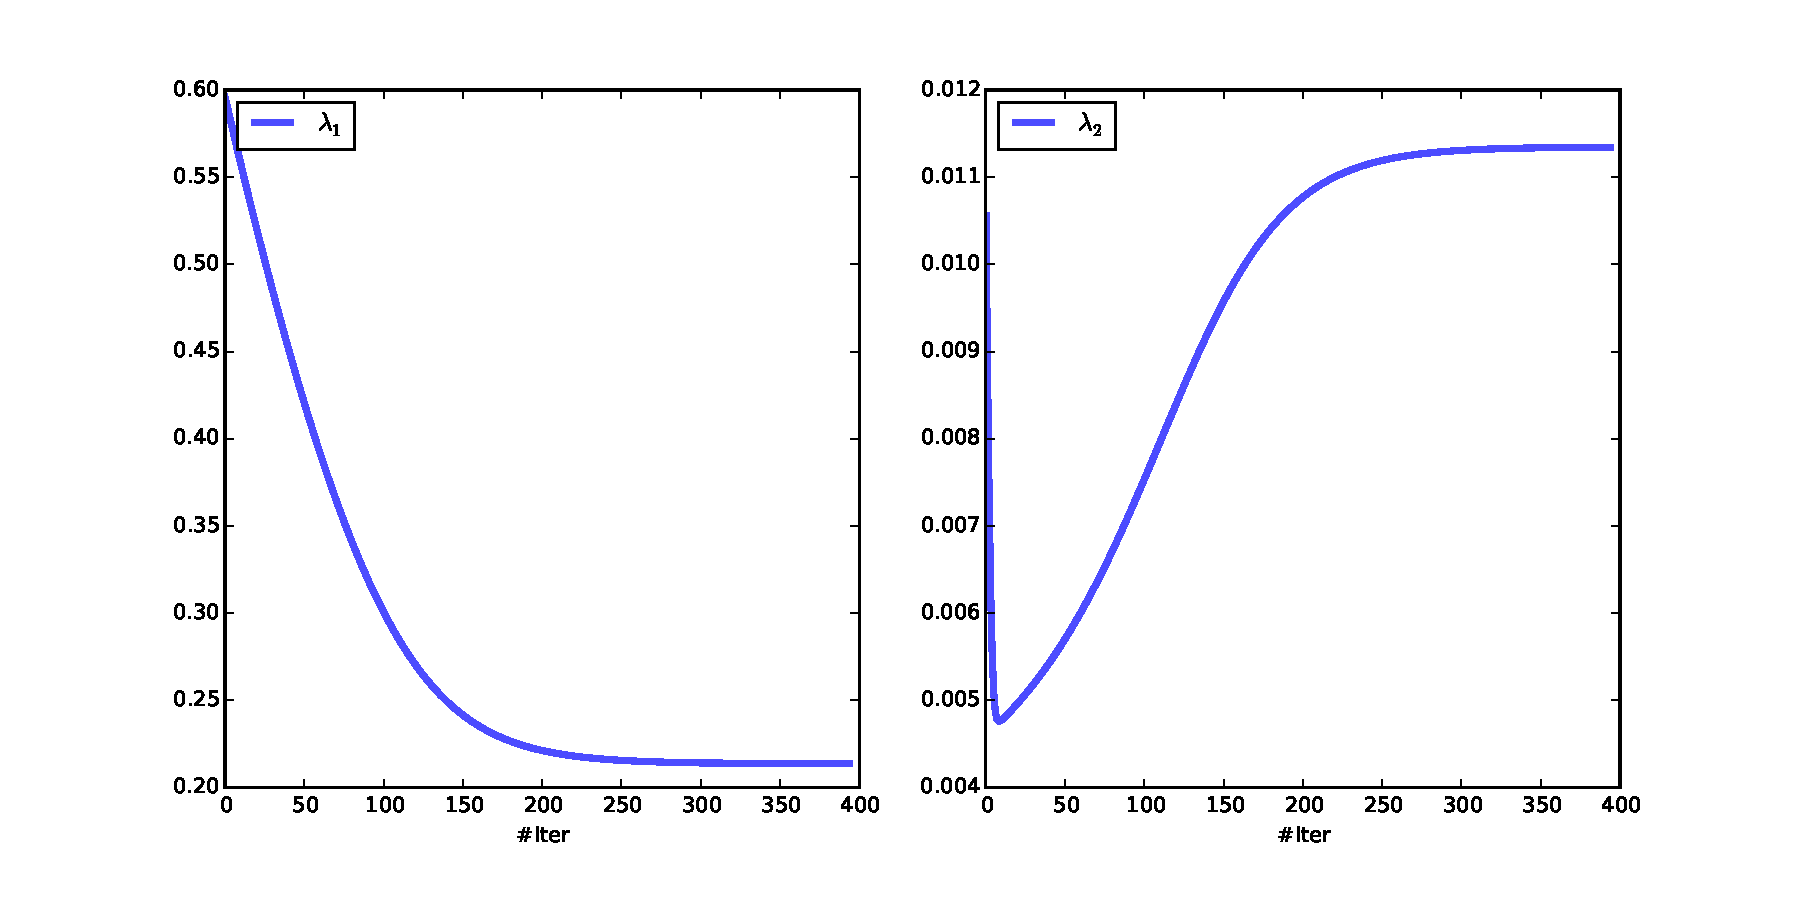
\includegraphics[width=6in]{graph/iter.pdf}
  \caption{Estimated $\lambda_1$ and $\lambda_2$}
  \label{est2}
\end{center}  
\end{figure}

After $400$ iterations, $\lambda_1$ and $\lambda_2$ converge to $0.2136$ and $0.01134$.

$\sigma_{i,j} \sim 10^0$

So $\lambda_1 : \lambda_2 \sigma_{i,j} \sim 10^1$, this is consistent with the result in Section~\ref{eth}. From this result, we can conclude our idea of modelling the spread of Ebola on the network is sensible.

\subsection{Model Validation}

\subsubsection{Validate the model with observed data}
We use the estimated $\lambda_1$ and $\lambda_2$ to do the estimation of Ebola outbreak for every time step(2 weeks) based on historical data. Fig.~\ref{espread} shows the result of the estimation. The estimated values match well with the ground truth, thus, our model is valid.

\subsubsection{Validate the model with case study}
In the previous section, we showed our model fits very well with the data. Thus, our model is good at tracking the progress of the disease in one area. 

Apart from that, our model has strong predictive abilities because it is built on the network.

We obtained the real data to estimate which areas are prone to be transmitted.

We did a case study on the prediction of our model. 

For example, from observing the data till week 7 since the outbreak, our model produced prediction that there will be outbreak in Freetown and Port Loko. Then in week 8, those two areas are infected indeed. Moreover, the news\cite{ebolanew} confirmed that the outbreak of Ebola in Freetown and Port Loko is due to transmission from adjacent areas.


\begin{figure}[hbtp]
\begin{center}
  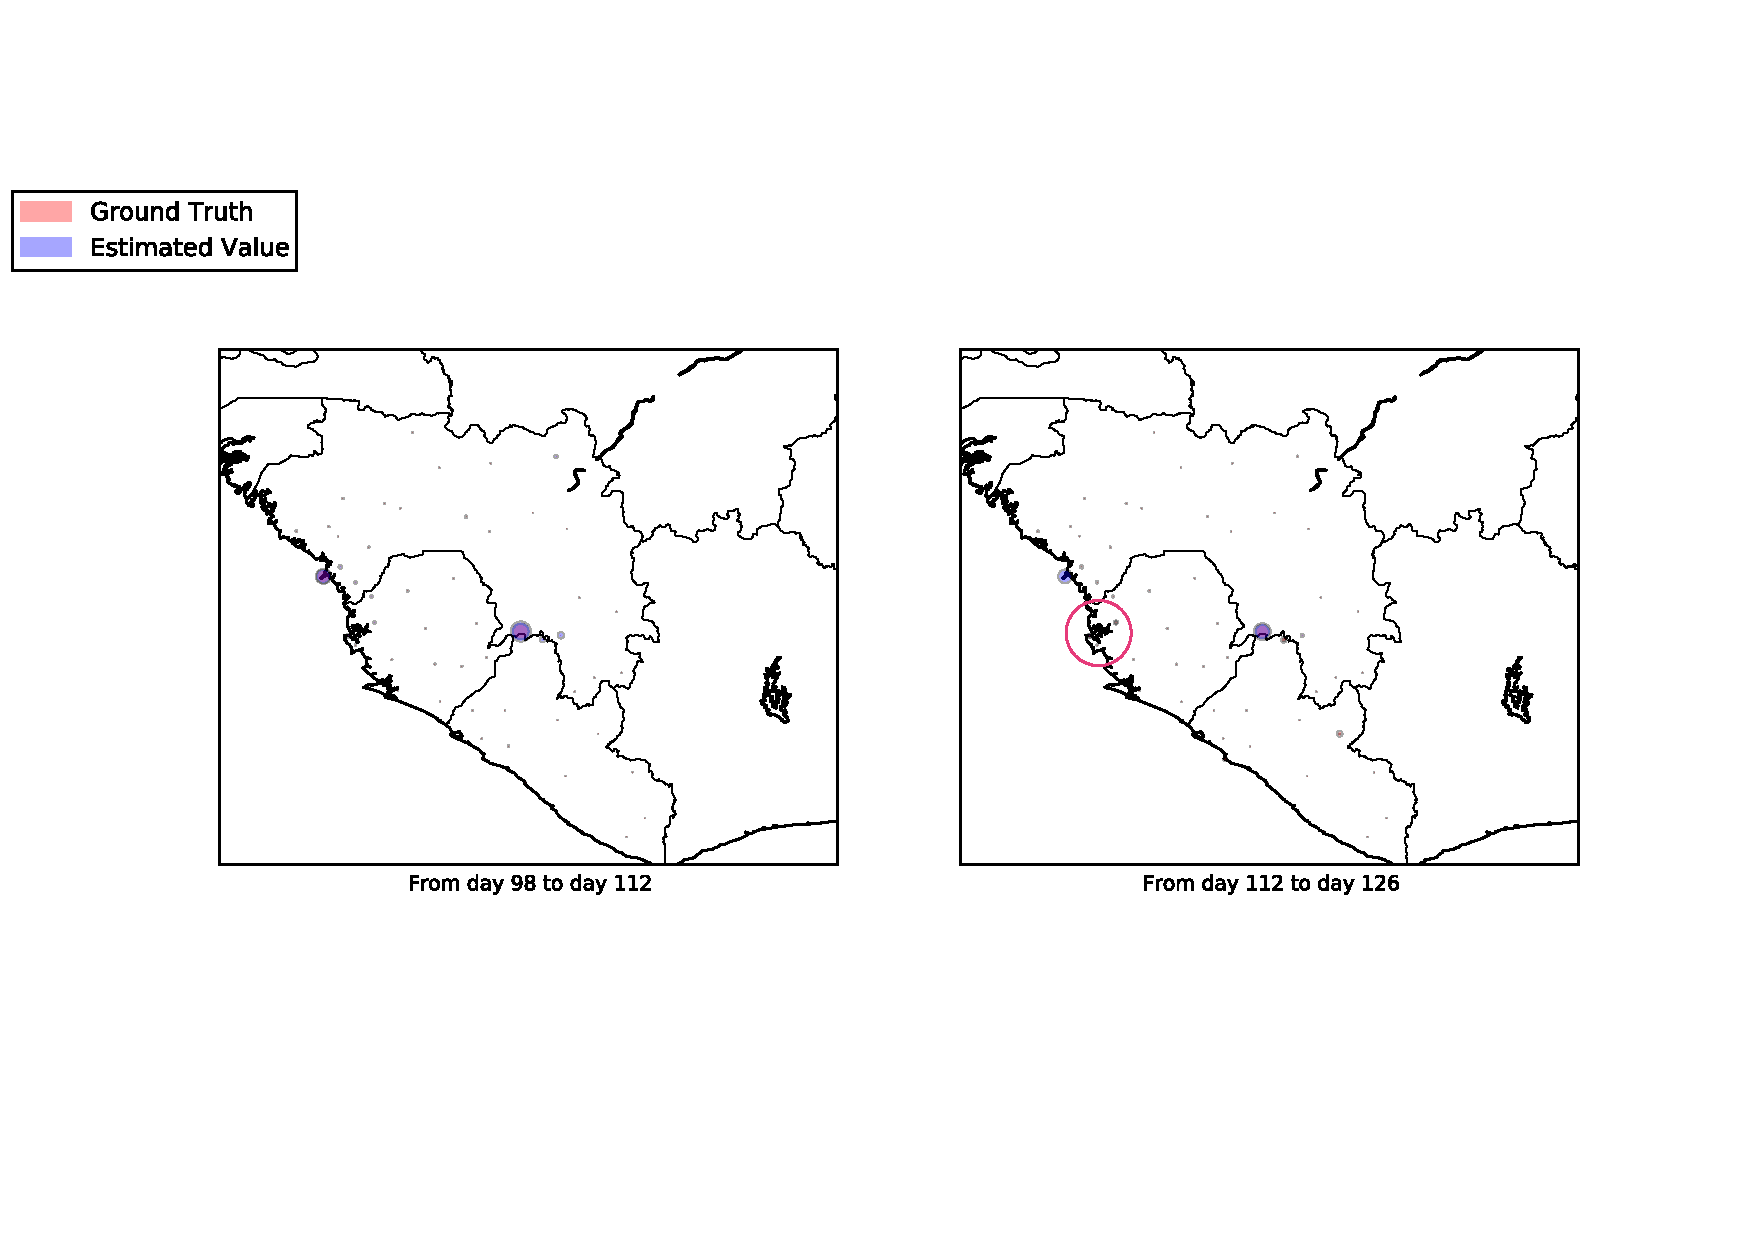
\includegraphics[width=5.5in]{graph/est22.pdf}
  \caption{Estimated outbreak in Freetown and Port Loko}
  \label{est22}
\end{center}  
\end{figure}




\subsection{Model Analysis}

\subsubsection{Sensitivity analysis}

To evaluate the sensitivity of our model, we tested the effect $\beta$ on parameter learning. 


\begin{table}[hbtp]
\begin{center}
\begin{tabular}{|c|c|c|c|}
\hline
$\beta$ & $\lambda_1$ & $\lambda_2 $ & $\lambda_1 /\lambda_2 $  \\
\hline
0.04 &0.156878175309 & 0.0103198999254 & 15.201520988\\
\hline 
0.05 & 0.168281029925 & 0.0110653981448 & 15.20786037\\
\hline 
0.1 & 0.239070310929 & 0.0156758779473 & 15.250840287\\ 
\hline 





\end{tabular}
\end{center}
\caption{Results of proposed model }
\label{testtable}
\end{table}
 

It is natural for $lambda_1$ and $\lambda_2$ to decrease when $\beta$ increase, because the influence from previous time step decreases when $\beta$ increase. However $\lambda_1 /\lambda_2 $ remains constant, so our model is robust.

Then We test our model against another parameter $wd$, this parameter is used to trim the exponential decaying kernel. For $wd = \infty$, we consider all historical data, for $wd = k$, we only consider previous $k$ time steps.





\begin{table}[hbtp]
\begin{center}
\begin{tabular}{|c|c|c|c|}
\hline
$wd$ & $\lambda_1$ & $\lambda_2 $ & $\lambda_1 /\lambda_2 $  \\
\hline
1 &0.168281029925 &0.0110653981448 & 15.20786037\\
\hline 
3 & 0.170180726118 & 0.0108785370316 & 15.643714373\\
\hline 
$\infty$  & 0.21365953932028273 & 0.01134447988647677 & 18.833788896\\ 
\hline 




\end{tabular}
\end{center}
\caption{Sensitivity of proposed model }
\label{testtable}
\end{table}

So our model is relatively stable against parameter $wd$.

\subsubsection{Prediction abilities analyisis}

We experimented on the prediction ability of our model. For each time step, we will predict a value for each region that is not yet infected. 

We used a threshold to determine whether there will be an outbreak. We calculated the false positive, false negative, true positive and true negative for our predictions. 

Fig.~\ref{roc} and Fig.~\ref{acc} and shows the receive operating curve of the prediction task. The prediction result is good and is already validated by case study. 

\label{pa}
\begin{figure}[hbtp]
\begin{center}
  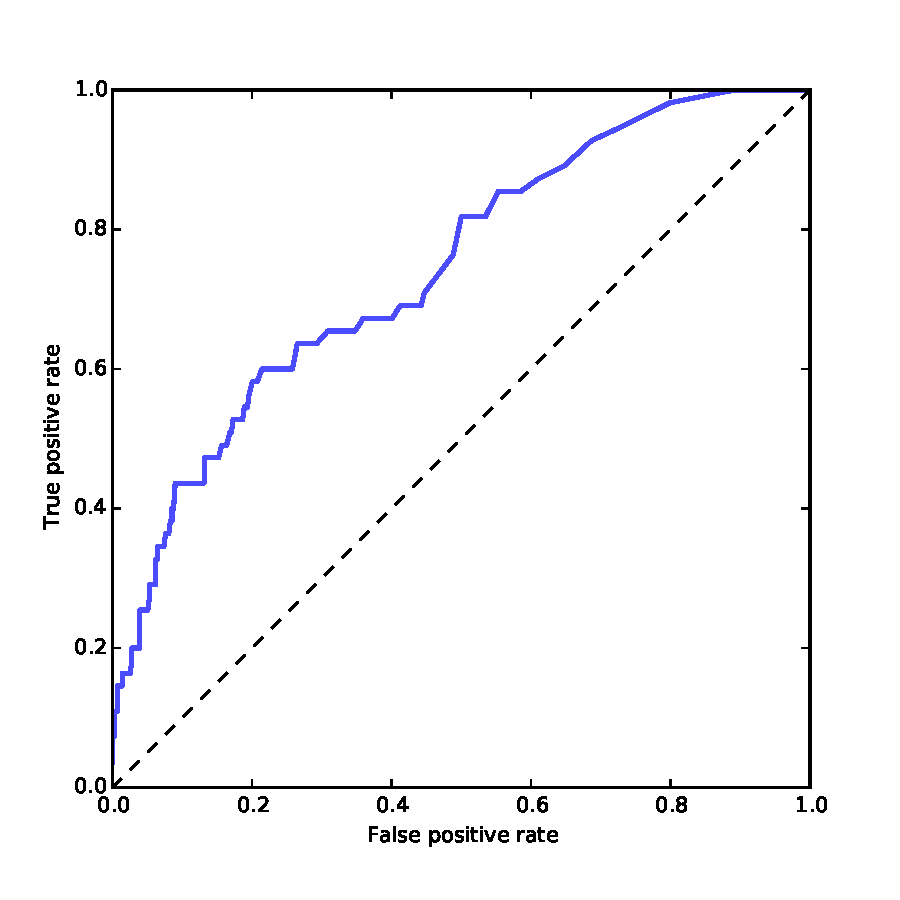
\includegraphics[width=3in]{graph/roc.pdf}
  \caption{ROC of prediction}
  \label{roc}
\end{center}  
\end{figure}

\begin{figure}[hbtp]
\begin{center}
  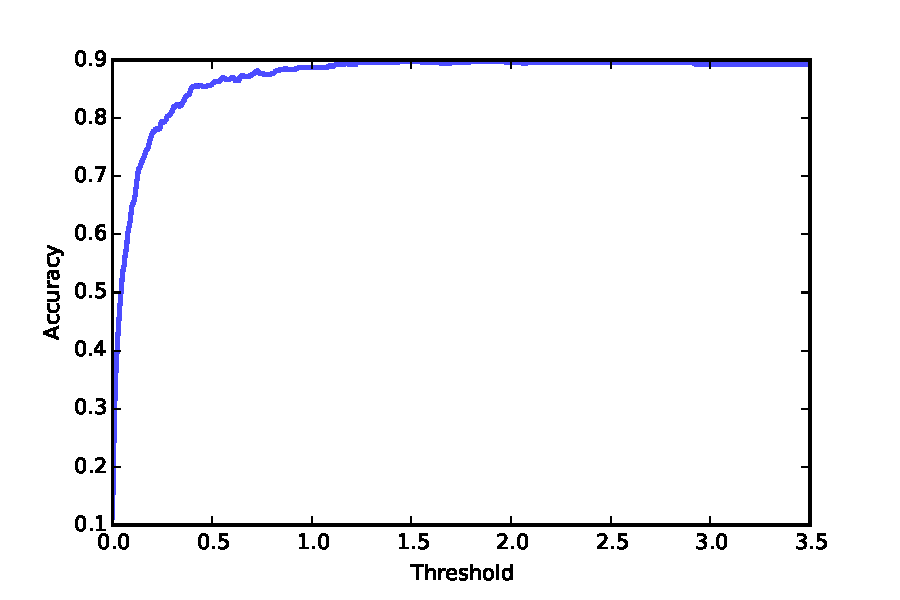
\includegraphics[width=3in]{graph/acc.pdf}
  \caption{Accuracy of prediction}
  \label{acc}
\end{center}  
\end{figure}



\begin{figure}[hbtp]
\begin{center}
  
\includegraphics[width=1in]{graph/elabel.pdf}

  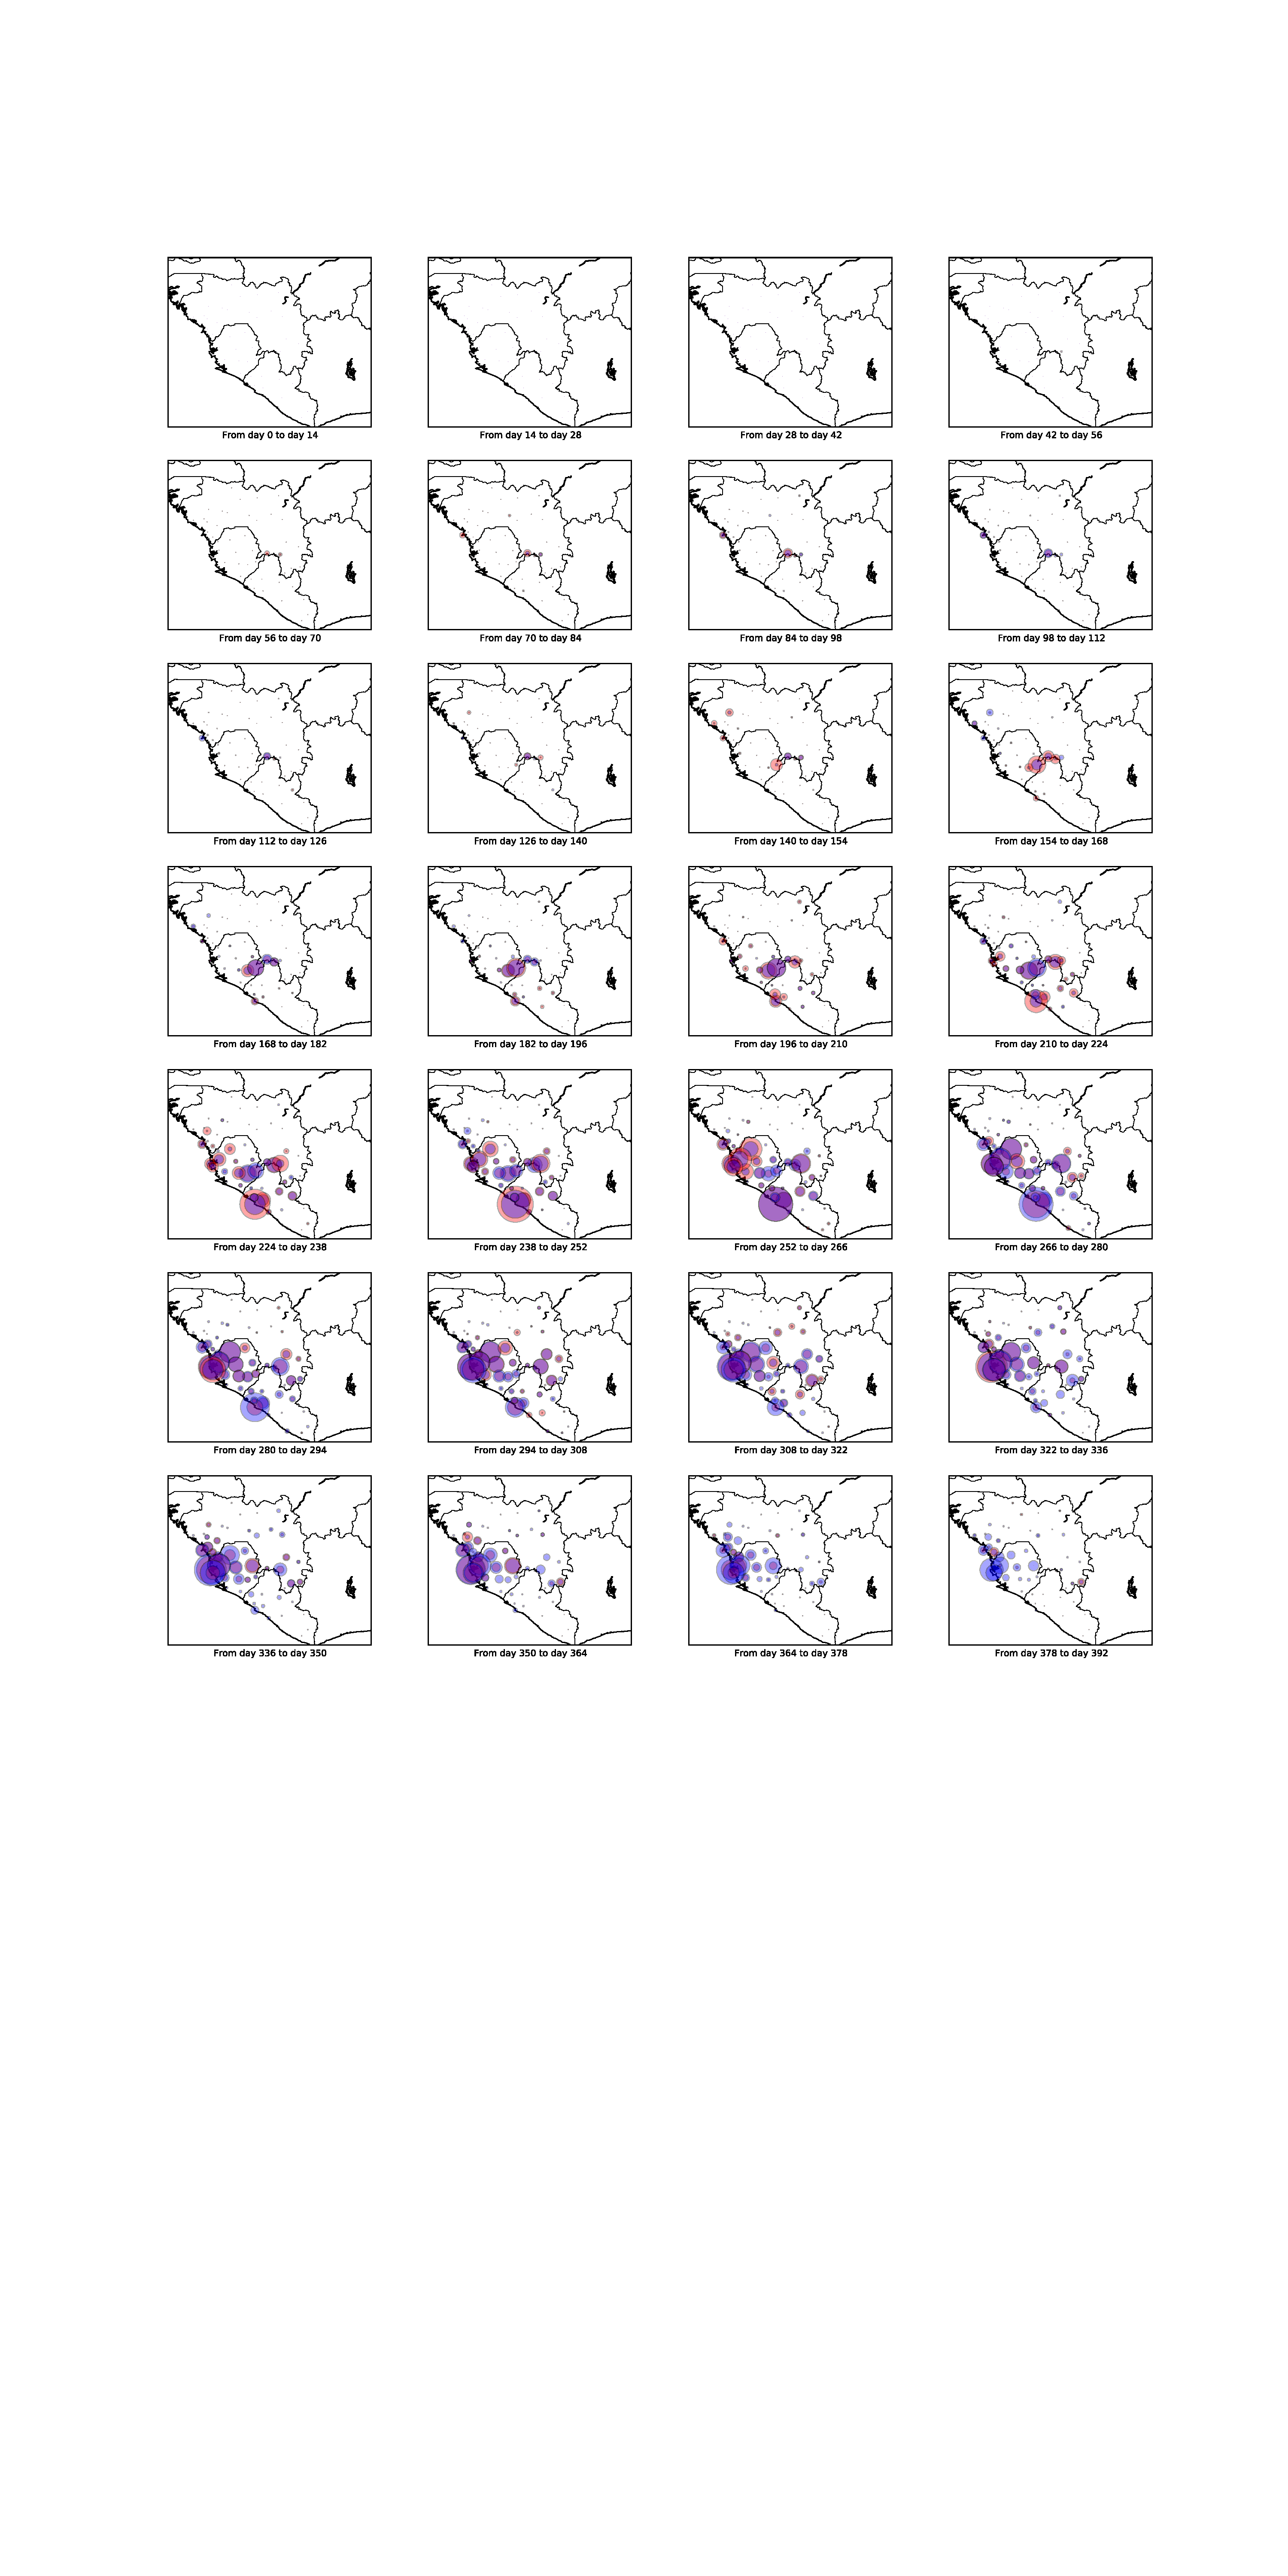
\includegraphics[width=5.9 in]{graph/ee.pdf}
  \caption{Estimated spatiotemporal spread of Ebola. The red marker means the ground truth and the blue marker means the estimated value. And the area of the circle means the scale of the outbreak. For the well estimated outbreaks, the two colors mix to make purple.}
  \label{espread}
\end{center}  
\end{figure}


\section{Disease Controlling}

\subsection{Objective}
We break the control of the disease into two steps with considering different factors. 

The first step is to temporarily bring the Ebola under control. We formalize this problem as following:

\emph{Problem~1:}

Given the Ebola spread models in Section~\ref{dmodel}, and a certain medication model $M$, with the current situation $P_{j,t_m}, j \in V, t_m \leq T$. Propose the best allocation of medicine, to minimize the loss $L(T')$ at time $T'$, $T' > T$, and determine the impact of important factors to the disease controlling process.


\emph{Problem~2:}

The second step is to ultimately eliminate the Ebola disease from the earth. This goal is formalized as following:

Given the Ebola spread models in Section~\ref{dmodel}, and a certain medication model $M$, with the current situation $P_{j,t_m}, j \in V, t_m \leq T$. Propose the best allocation of medicine, to minimize the cumulative loss $\int_{T}^{\infty} L(t) dt $, and determine the critical factors having effect on whether   the disease can be eliminated, i.e, $\text{lim}_{t\rightarrow \infty} L(t) = 0 $

For different perspectives in Problem $1$ and $2$, either proposed disease spreading model has advantages, so we will use the most suitable model for  analysing different tasks in those problems.


\subsection{Disease Controlling based on CasPPonNET}

\label{str}

\subsubsection{Drug allocation based on CasPPonNET}
The mechanism of medicine on a patient $P$ : If the disease is not advanced (less than $T_0$), $P$ is recovered and removed from the system. And $P$ will not have any effects on the next time step.

We set $T_0$ to two weeks. 

If the observation window is long, for example if $\Delta t= T_0$, then only patients in last time step can be cured.

Assume we have $m$ amount of medicines for $m$ patients. And we want to maximize the effect of these medicines.

$$\mu_{i,t_k} = \lambda_1 \sum_{m = 1}^{ k-1} P_{i,t_m} e^{-\beta(k-m)\Delta t} + \lambda_2 \sum_{j:j\neq i} \sum_{m = 1}^{ k-1} P_{j,t_m} \sigma_{j,i} e^{-\beta(k-m)\Delta t}$$

Denote $C_{i,t_m}$ is the number of patients cured in area $i$ and time step $m$, $C_{i,t_m} \leq P_{i,t_m}$.

$$\sum_i C_{i,t_m} = C_{t_m}$$

$$\mu'_{i,t_k} = \lambda_1 \sum_{m = 1}^{ k-1} (P_{i,t_m} - C_{i,t_m}) e^{-\beta(k-m)\Delta t} + \lambda_2 \sum_{j:j\neq i} \sum_{m = 1}^{ k-1} (P_{j,t_m}-C_{i,t_m}) \sigma_{j,i} e^{-\beta(k-m)\Delta t}$$

$$
E[\sum_n {P'_{n,t_k}}] = \sum_i \mu'_{i,t_k} = \lambda_1 \sum_n \sum_{m = 1}^{ k-1} P'_{i,t_m} e^{-\beta(k-m)\Delta t} + \lambda_2 \sum_n \sum_{j:j\neq i} \sum_{m = 1}^{ k-1} P'_{j,t_m} \sigma_{j,i} e^{-\beta(k-m)\Delta t}
$$
$$
\lambda_1 \sum_n \sum_{m = 1}^{ k-1} (P_{i,t_m} - C_{i,t_m}) e^{-\beta(k-m)\Delta t} + \lambda_2 \sum_n \sum_{j:j\neq i} \sum_{m = 1}^{ k-1} (P_{j,t_m} - C_{i,t_m}) \sigma_{j,i} e^{-\beta(k-m)\Delta t}
$$

The coefficient of $C_{i,t_m}$ is $-$$\lambda_1 e^{-\beta(k-m)\Delta t} - \lambda_2 \sum_{j:j\neq i} e^{-\beta(k-m) \Delta t}$



Then we find the node with the max weight:
 $$w_{c,i} = \lambda_1 + \lambda_2 \sum_{j:j\neq i} \sigma_{j,i}$$
 
In this case, the weight of areas is only related to $\sum_{j:j\neq i} \sigma_{j,i}$.


If the observation window is smaller, for example $\Delta t = \frac{1}{u} T_0$, then patients in last $u$ time steps can be cured. 

$$w_{c,i,m} = \lambda_1 e^{-\beta(k-m)\Delta t} + \lambda_2 \sum_{j:j\neq i} e^{-\beta(k-m) \Delta t}, k-u\leq m < k$$

\label{421}

\emph{Allocation Strategy:}

First satisfy the needs of areas with highest $w$.

If the patients are all cured in an area, deliver the drugs to the area with the next highest $w$.

\subsubsection{Vaccine allocation based on CasPPonNET}


Vaccination:

The vaccination is applied to a number of citizens in a certain area $i$ at a certain time $t_m$, then they are immune to Ebola in the future $t,t>t_m$. 

$$Va_{i,t_m} = \delta Po_i $$
$$\sum_i Va_{i,t_m} = Va_{t_m} $$
 

Then 
$$\mu'_{i,t_k} =(1 - \delta) \mu_{i,t_k} , k > m $$ 


$$
E[\sum_{i \in n} {P'_{n,t_k}}] = \sum_{i \in n} \mu'_{i,t_k} = \lambda_1 \sum_{i \in n} \left( 1 - \frac{Va_{i,t_{ < k}}}{Po_i} \right) \sum_{m = 1}^{ k-1} P_{i,t_m} e^{-\beta(k-m)\Delta t} $$
$$ + \lambda_2 \sum_{i \in n}\left( 1 - \frac{Va_{i,t_{< k}}}{Po_i}\right) \sum_{j:j\neq i} \sum_{m = 1}^{ k-1} P_{j,t_m} \sigma_{j,i} e^{-\beta(k-m)\Delta t}
$$

The benefit from $Va_{i,t_{ < k}}$ is:

$$
w_{v,i} = \lambda_1 \sum_{m = 1}^{ k-1} \frac{P_{i,t_m}}{Po_{i}} e^{-\beta(k-m)\Delta t} + \lambda_2 \sum_{j:j\neq i} \sum_{m = 1}^{ k-1} \frac{P_{j,t_m}}{Po_{i}} \sigma_{j,i} e^{-\beta(k-m)\Delta t} = \frac{E[P_{i,t_k}]}{Po_{i}}
$$
\label{422}


\emph{Allocation Strategy:}

First satisfy the needs of areas with highest $w$.

If the population are all vaccinated in an area, deliver the drugs to the area with the next highest $w$.

\subsubsection{Drug/Vaccine delivery system}

When we consider the cost of transport in practical cases, all we need to do is to add resistance on each edge of the network. We can then describe it mathematically by adding a constraint to the optimization problem we describe in \ref{421} and \ref{422}. What's more, if the resistance is proportional to the transport quantity, the weight of each node in transportation can be estimated.

\subsubsection{Experimental validation}

We adopted the strategy in Section \ref{str} to test their effects on disease controlling.

We tested the proposed method against other trivial methods such as assign medicine proportional to number of new cases and showed our method is optimal.

If the number of medicine is fixed, it can be inferred from Figure.\ref{med} that no matter how much the amount of the drug is, our strategy is always the best.

In Figure.~\ref{ev}, we tested the proposed vaccination method against other general methods such as assign vaccine proportional to number of new cases and showed our method is optimal.

We can draw a conclusion from Figure.~\ref{med2} that when the amount of vaccine is a constant number. On the scale of the amount, our proposed vaccination method is better than other methods.




\begin{figure}[hbtp]
\begin{center}
  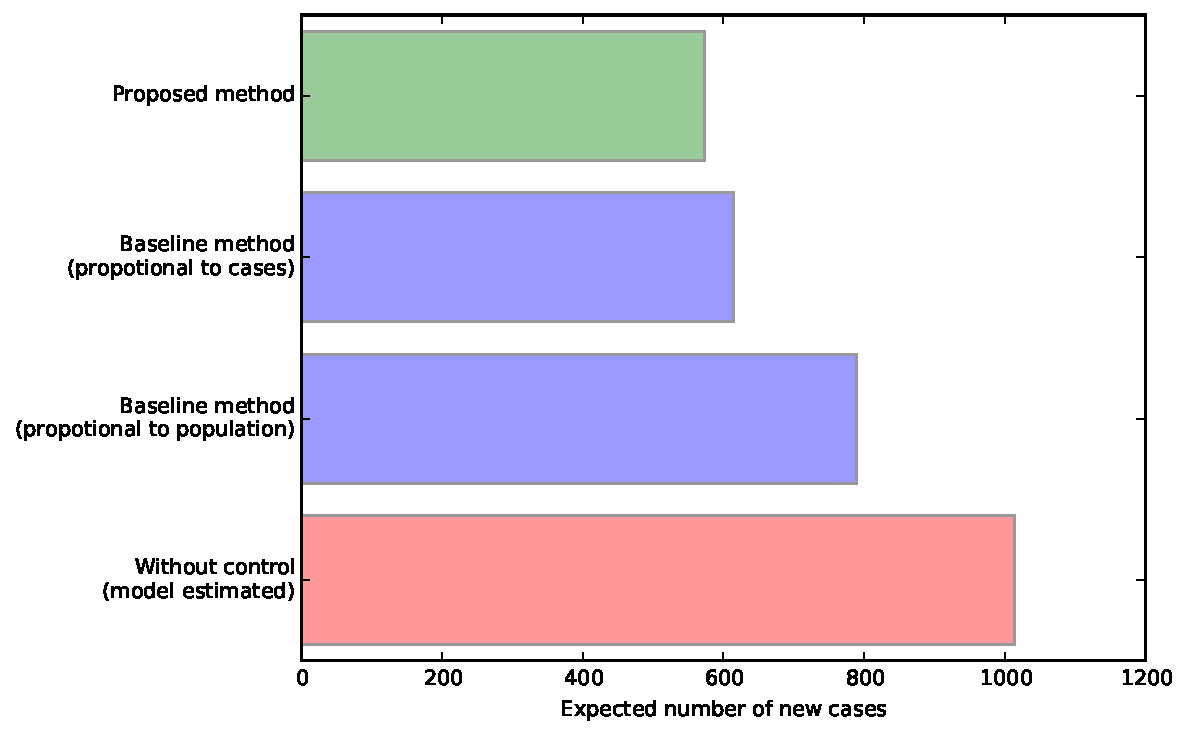
\includegraphics[width=3.5in]{graph/res2.pdf}
  \caption{Effect of different medication strategies}
  \label{med}
\end{center}  
\end{figure}


\begin{figure}[hbtp]
\begin{center}
  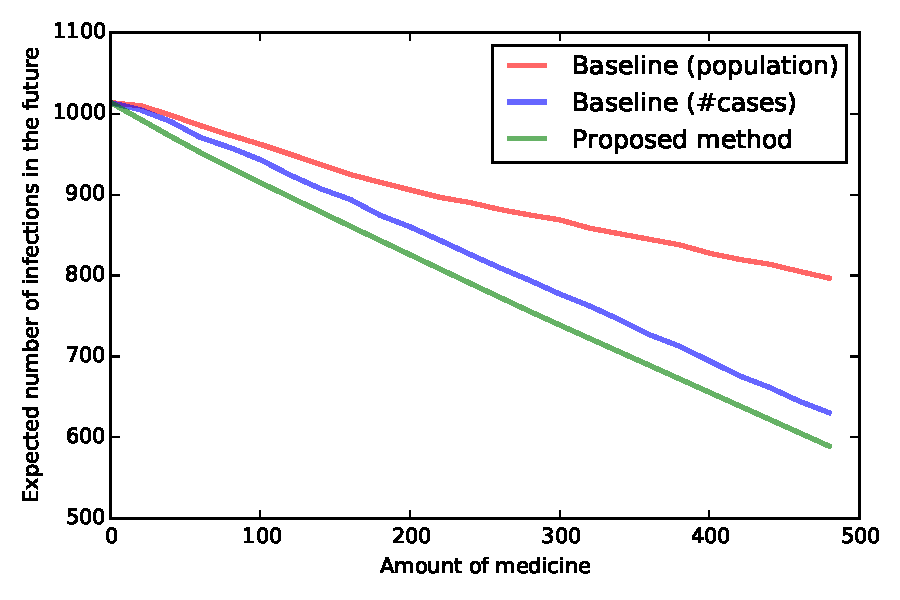
\includegraphics[width=3.5in]{graph/ev.pdf}
  \caption{Effect of different medication strategies over time}
  \label{ev}
\end{center}  
\end{figure}



\begin{figure}[hbtp]
\begin{center}
  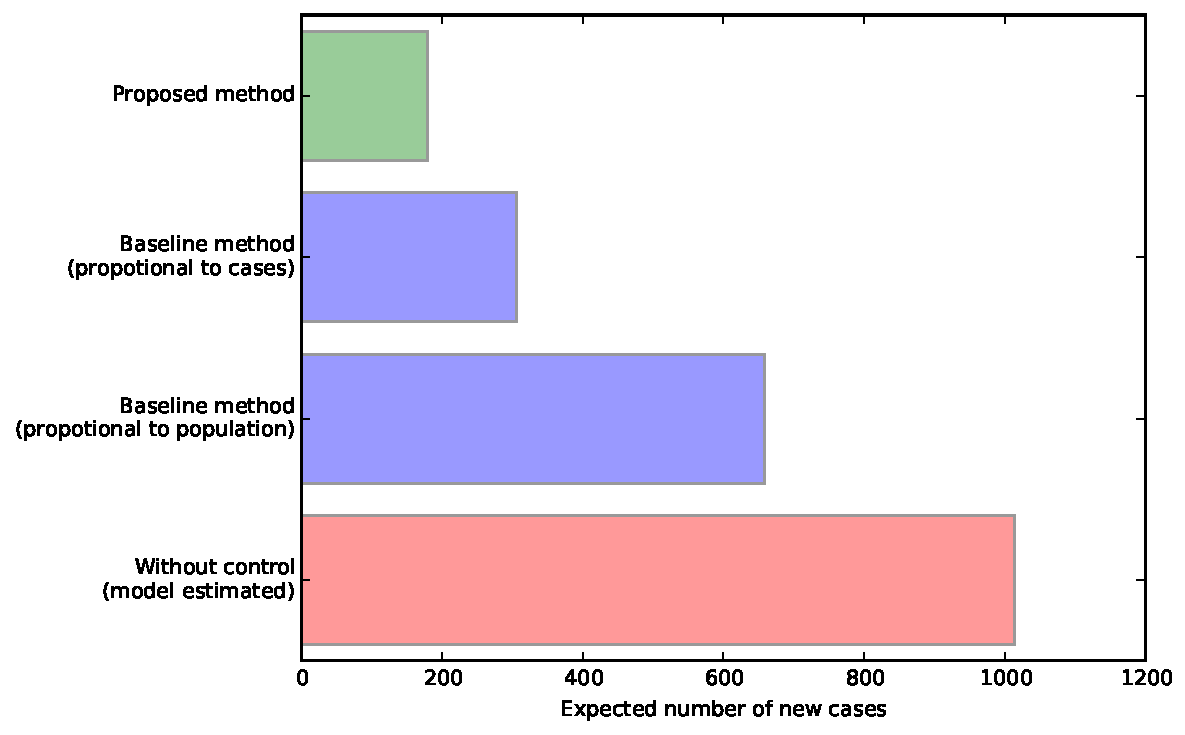
\includegraphics[width=3.5in]{graph/res4.pdf}
  \caption{Effect of different vaccination strategies}
  \label{med2}
\end{center}  
\end{figure}



\begin{figure}[hbtp]
\begin{center}
  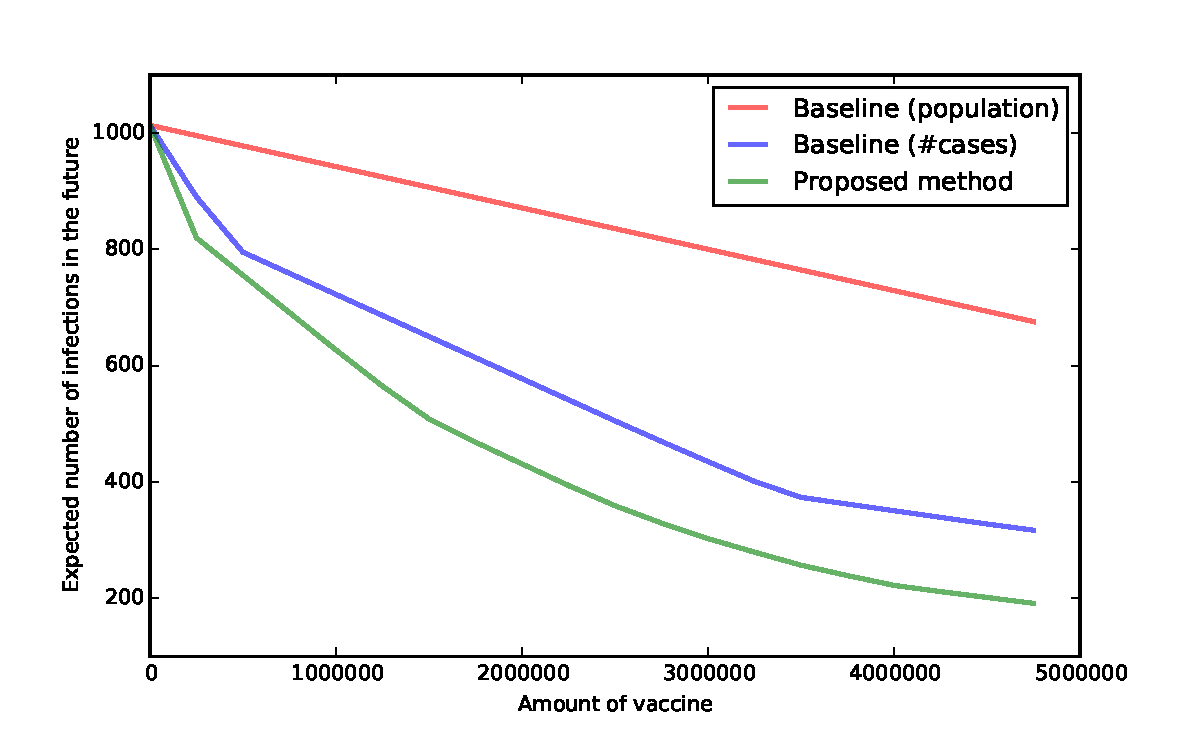
\includegraphics[width=3.5in]{graph/ev2.pdf}
  \caption{Effect of different vaccination strategies over time}
  \label{ev2}
\end{center}  
\end{figure}


\subsubsection{Realistic Results}

In order to produce realistic results to assist controlling the disease. We fed the real world data into our model and calculated $w_c$ and $w_v$ and the ranking of areas. This indicate how needed an area is for medicine or vaccine. 

As for $w_v$, it is irrelevant to the disease progress and remains constant during the whole timespan.

However, for $w_m$, it depends on the current situation. So we calculated them for a typical time week $34$ when disease began to spread in large scales and \emph{now} (Feb 9 2014).

The results are shown in Table~\ref{testtable}.

\begin{table}[hbtp]
\begin{center}
\begin{tabular}{|c|c|c|c|}
\hline

Rank & Need medicine & Need vaccination(week 34) & Need vaccination(now) \\
\hline
1 &Freetown(SL) &Lofa(LR) &Dubreka(GN) \\
\hline
2 &Conakry(GN) &Margibi(LR) &Forecariah(GN) \\
\hline
3 &Western rural(SL) &Dubreka(GN) &Western rural(SL) \\
\hline
4 &Port loko(SL) &Bong(LR) &Lola(GN) \\
\hline
5 &Kenema(SL) &Grand bassa(LR) &Coyah(GN) \\
\hline
6 &Bo(SL) &Bomi(LR) &Freetown(SL) \\
\hline
7 &Kambia(SL) &Montserrado(LR) &Port loko(SL) \\
\hline
8 &Montserrado(LR) &Macenta(GN) &Kambia(SL) \\
\hline

\end{tabular}
\end{center}
\caption{Results of proposed model}
\label{testtable}
\end{table}





\subsection{Determination of Manufacturing rate }

The manufacturing rate plays an important role in the disease controlling process. In order for the disease to be controlled, the $E[\sum_{i \in n} {P'_{n,t_k}}]$
has to decay to zero.

For this objective, due to the complexity of the distribution of disease, a theoretical solution is hard to obtained. So we did experiments to determine the critical value.


In our simulation, $m$ represents the medicine which is put into the system per two weeks under the best disease controlling strategy. All the initial condition of simulation is set to be the same as that of the 34th week. 

Our simulation shows that different manufacturing rates do affect the evolution of the number of cases. When no or not enough medicine is manufactured, the EVD will be developed monotonically. In contrast, when sufficient supply of medicine is guaranteed, the disease will finally be defeated.

In order to find the singular point leading to the bifucation, a more detailed simulation is given and we find the least number of medicine manufacturing is about 52 per two weeks.  

It is easy to see that the earlier the medicine is putted into the West Africa, the more important role it will take. To simulate the time effect of the medicine delivery, we use a constant manufacturing rate but started at different time, we can see that even 100 per two weeks can not control the EVD when 38 weeks past.

\begin{figure}[hbtp]
\begin{center}
  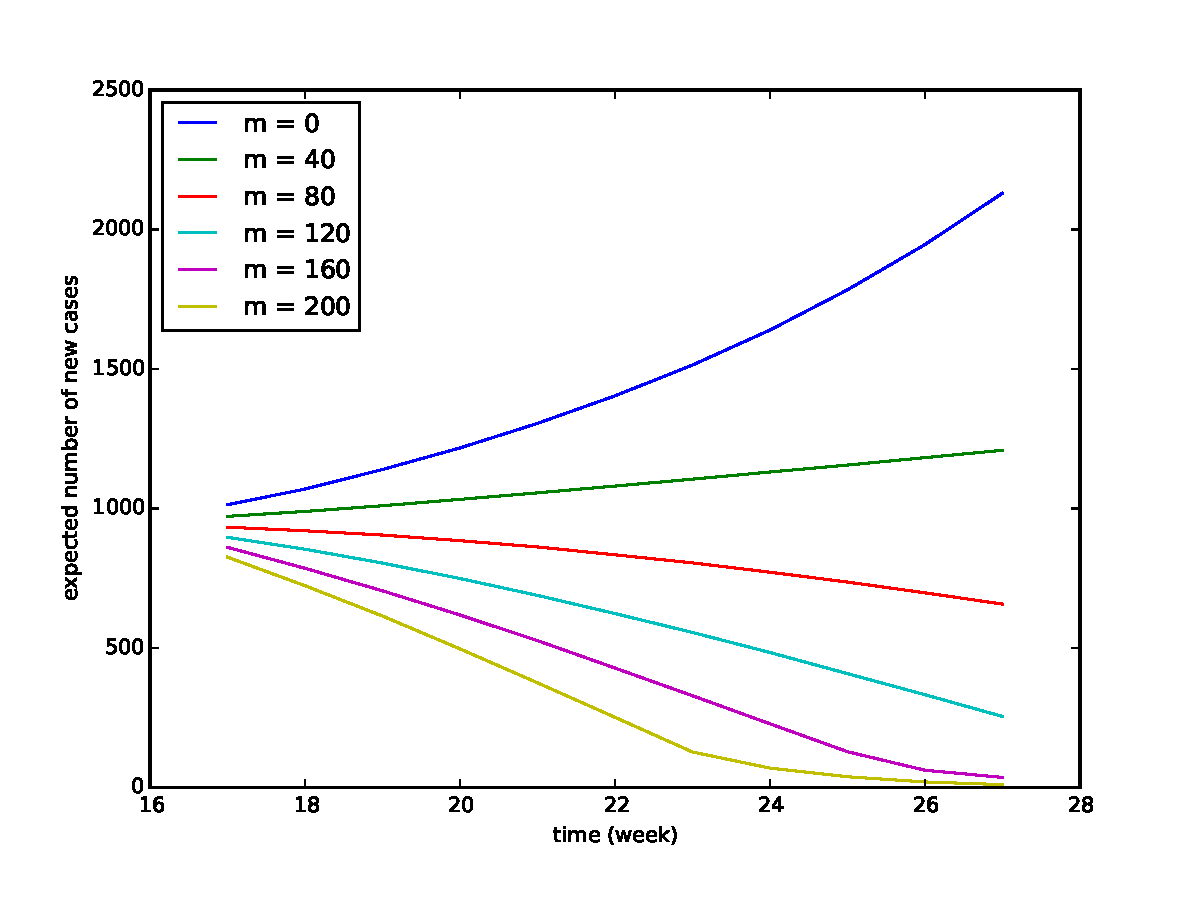
\includegraphics[width=4in]{graph/good.pdf}
  \caption{Comparison to random prediction}
  \label{g1}
\end{center}  
\end{figure}

\begin{figure}[hbtp]
\begin{center}
  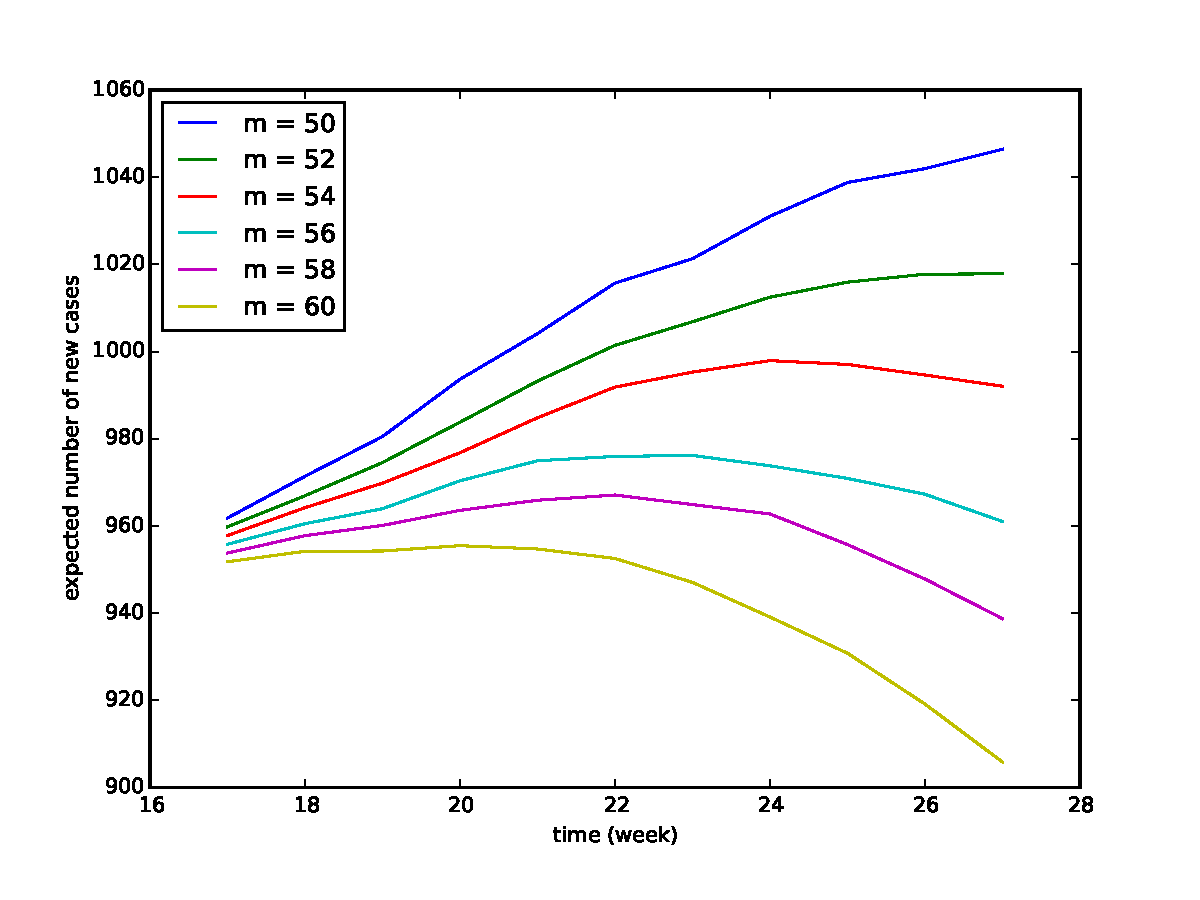
\includegraphics[width=3.5in]{graph/good2.pdf}
  \caption{Effect of different start time of medication}
  \label{g2}
\end{center}  
\end{figure}


\begin{figure}[hbtp]
\begin{center}
  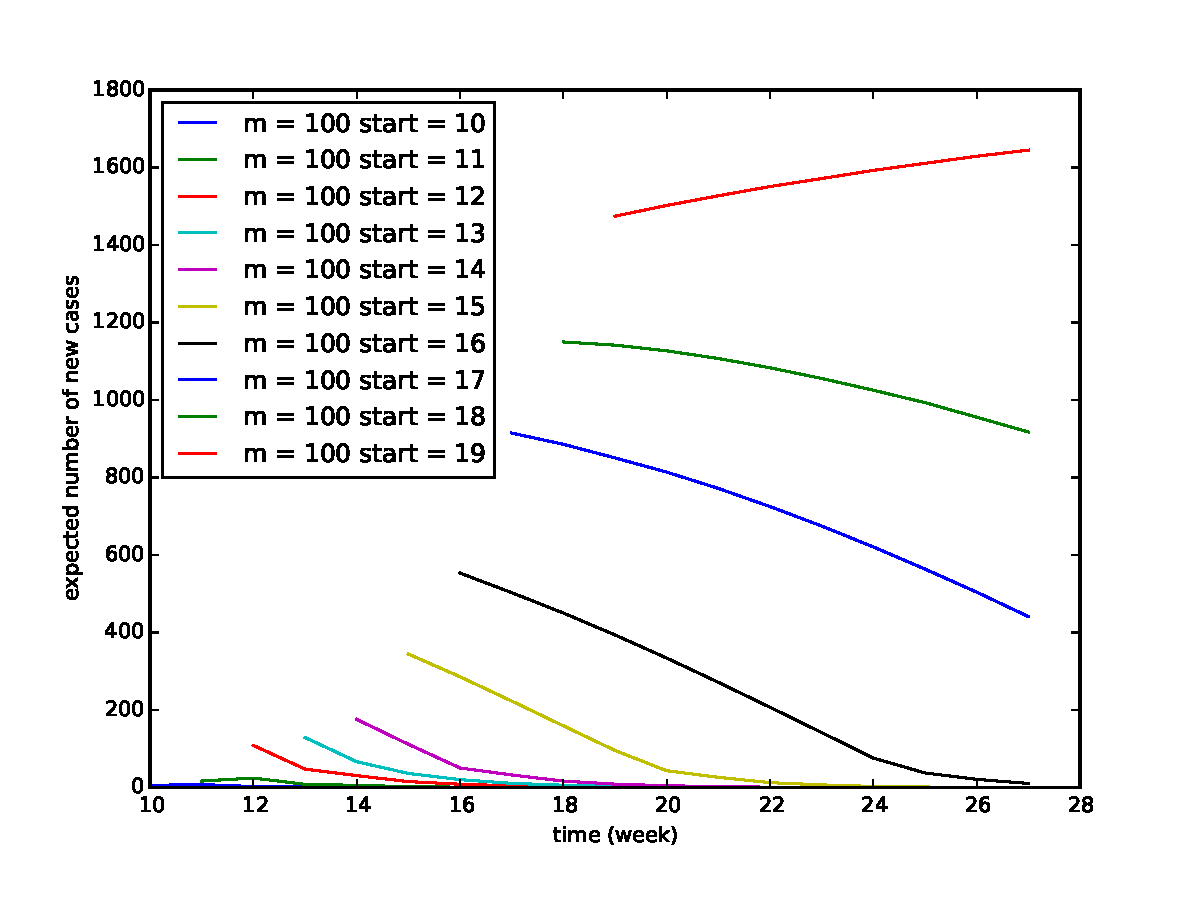
\includegraphics[width=3.5in]{graph/good4.pdf}
  \caption{Effect of different start time of medication}
  \label{g3}
\end{center}  
\end{figure}

 

\subsection{Disease Precautioning System}

Apart from drug and vaccine, other general precautions can be made to those regions which have risk of potential outbreak in the future. 

In section \ref{pa} we discussed that our model has strong abilities to predict future outbreak. 

We would like to use this prediction result to do precautions such as improving healthcare infrastructures. Without building a detailed model, we assume a certain \emph{cost} to false positive predictions and false negative predictions.

False negative predictions will have  heavy costs because it will lead to huge outbreaks.

False positive predictions will have small costs. 

$$Cost = g FN + FP$$

$g$ is the ratio of two different costs, $g >> 1$ and is determined empirically to optimize the threshold for alerting and precautioning system.

For example, in Fig~.\ref{random} we set $g = 8$ and the optimal value for threshold is $0.2$. The least cost is about $2/3$ the cost based on random guess.  



\begin{figure}[hbtp]
\begin{center}
  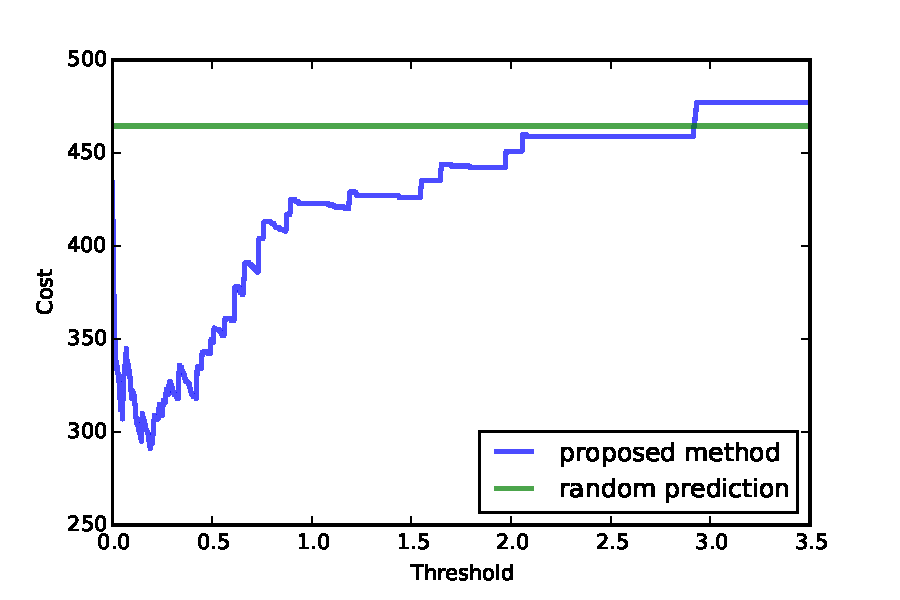
\includegraphics[width=3.5in]{graph/cost.pdf}
  \caption{Comparison to random prediction}
  \label{random}
\end{center}  
\end{figure}



\section{Discussions and Future works}

\subsection{ Superiority}
\begin{itemize}

\item 	Our model is based on geographical network, so it's a good method to model the Ebola's geographical spread due to people migration. We use the data to estimate our parameters. Then we can evaluate how important each term is.

\item 	A lot of our conclusions are based on the theoretical derivation, some assumptions also established in Ebola's characteristics. 

\item 	By comparing with other models especially SIHR, we can fully exploit its strengths in prediction and optimization. 


\end{itemize}


\subsection{ Weakness }
\begin{itemize}

\item	A data-driving model has a naturally problem: cold start. It is suitable for the infectious disease outbreak soon but not fully developed.

\item	Due to the restriction of computer simulation, some of our assumptions are highly ideal, such as the `Gravity Model' of population flow.
\end{itemize}


\subsection{Future Research}

\begin{itemize}

\item	If the medicines and drugs really exist. We can get a lot of data to test our model, to formulate the optimized strategies in many other independent variables.

\item	Some medical treatment such as isolation can have an unambiguous influence in our model. For example, exponential decay is faster than before. We will consider it in our model in an explicit way.

\item	Population migration determines the geographical spread of EVD, but the migration model based on the simple gravity model. If we have enough time to meditate, the output of the model will be more realistic.

\end{itemize}


\newpage
\bibliography{ref}
\bibliographystyle{ieeetr}


\newpage


\section*{Appendix}
\label{appendix}

\begin{enumerate}
\item The data is mainly from the WHO website. We also wrote a script to fetch the geographical data. 

%\item The code and data are available at \href{https://github.com/Eureka22/CasPPonNET}{https://github.com/Eureka22/CasPPonNET}

\item Some large figures are plotted in this section to save space for the main paper.
\end{enumerate}




\begin{figure}[hbtp]
\begin{center}
  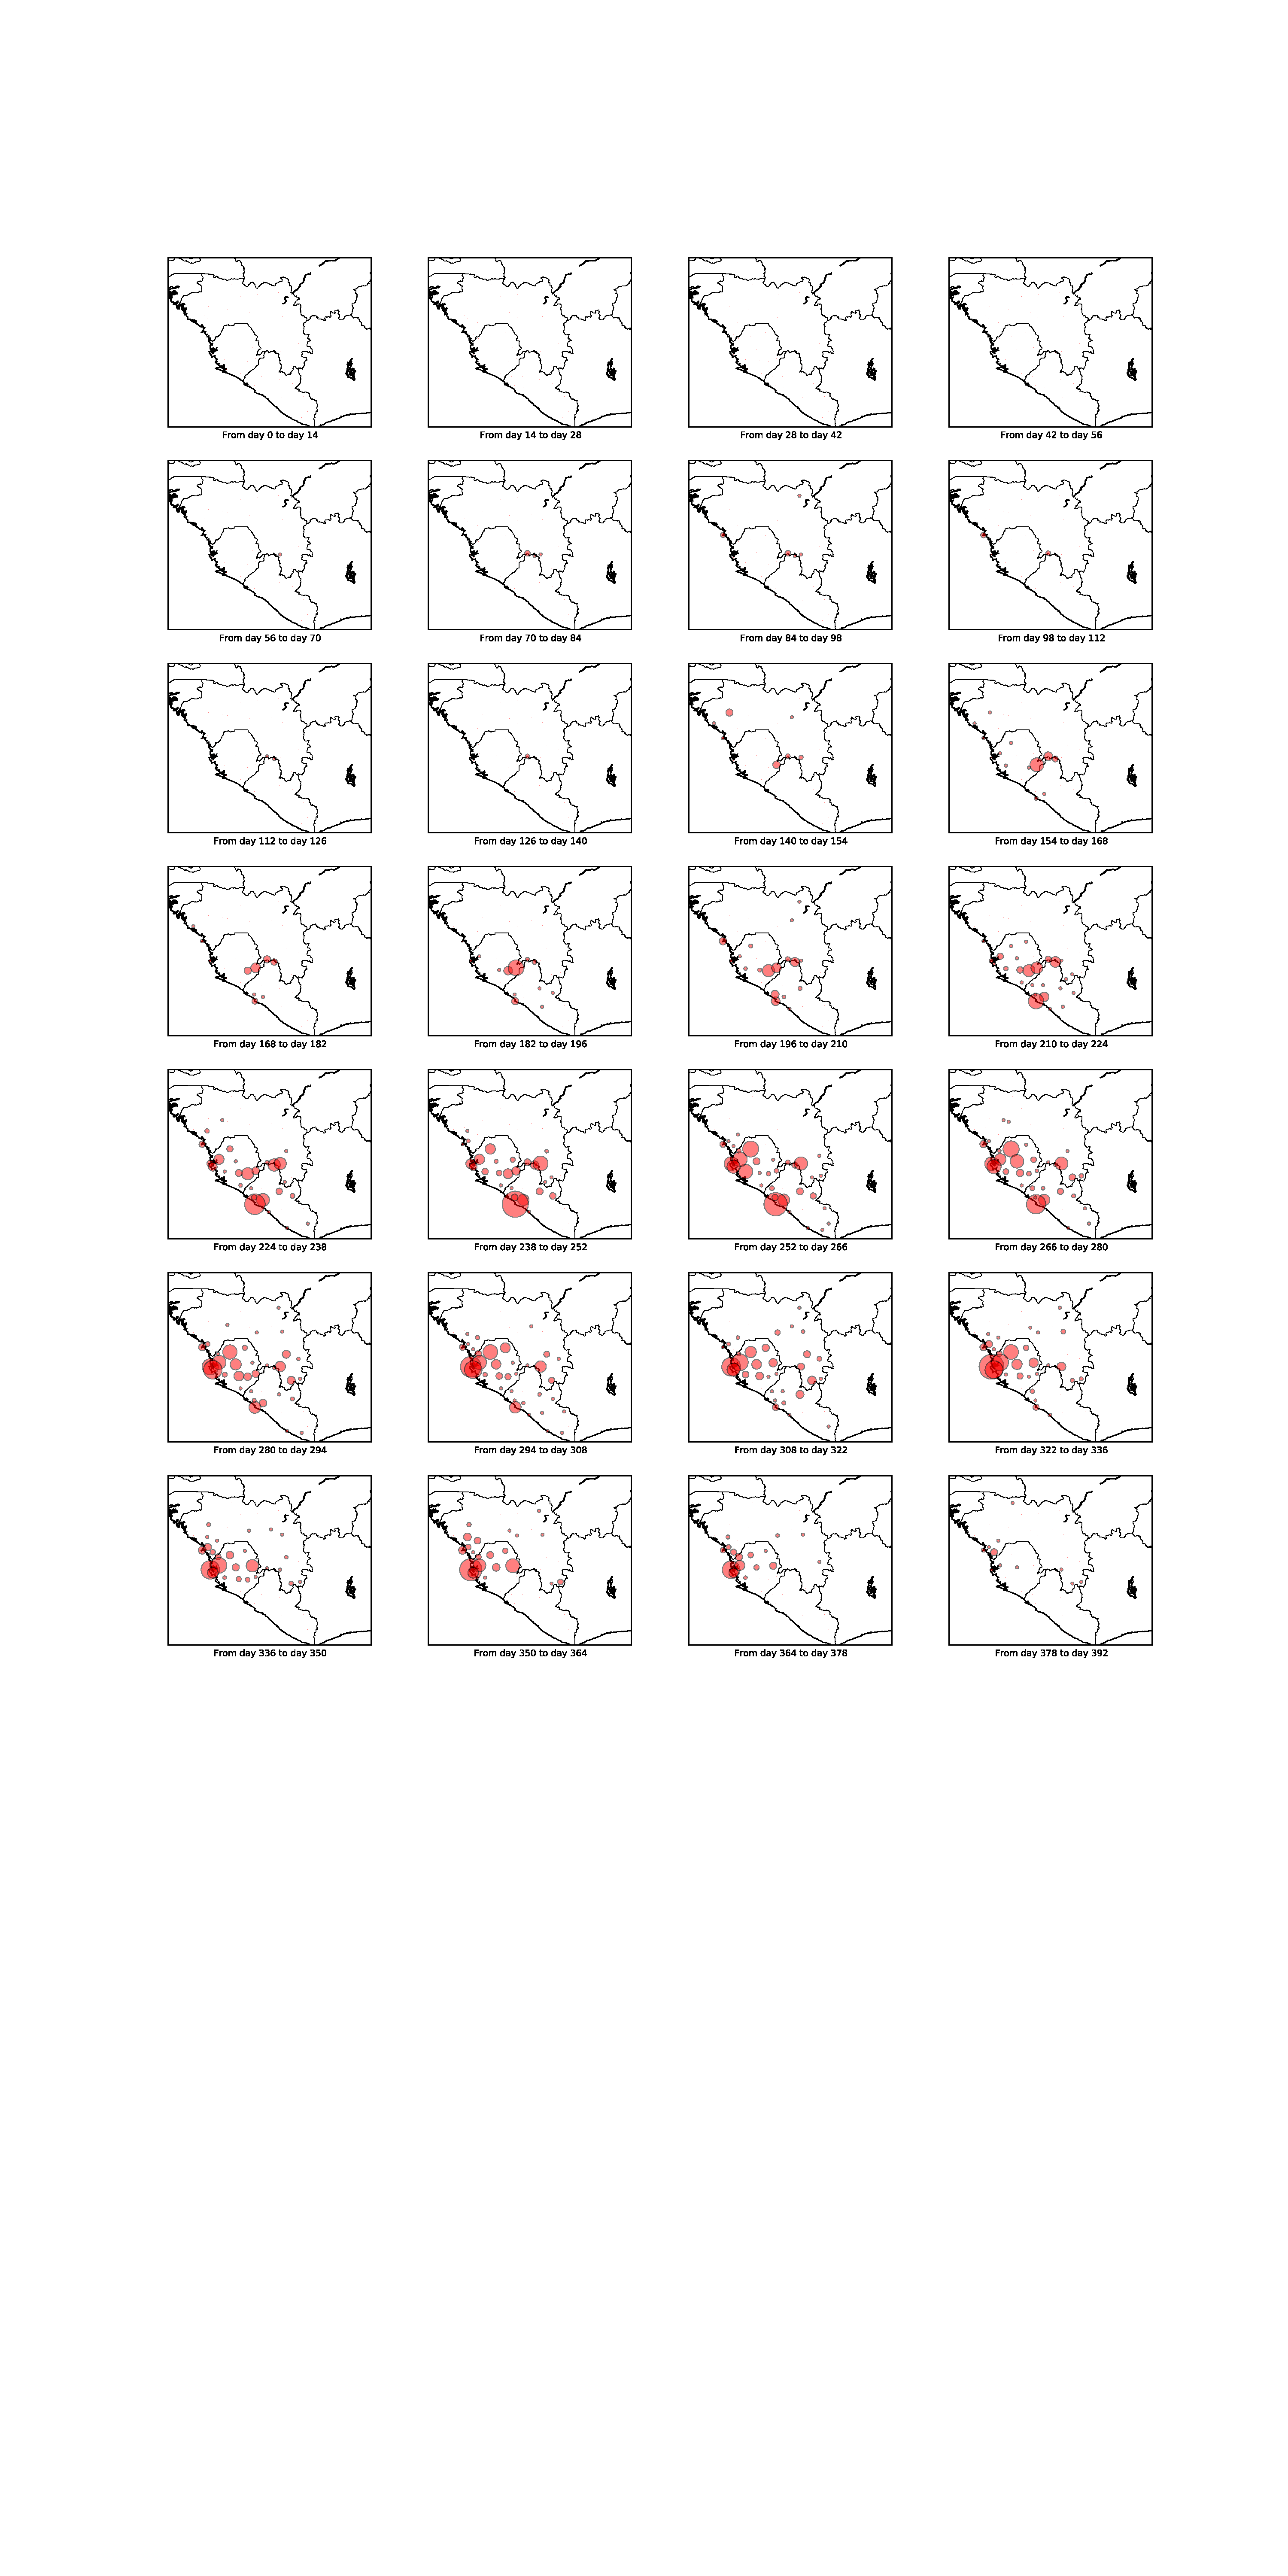
\includegraphics[width=6.1in]{graph/spread2.pdf}
  \caption{Spread of Ebola disease}
  \label{spread}
\end{center}  
\end{figure}

\label{lastpage}
\end{document}